\documentclass[a4paper,12pt]{report} % for final document
%\documentclass[draft, a4paper,12pt]{report} % for drafts

\usepackage[utf8]{inputenc}
\usepackage{graphicx}
\usepackage{amsmath}
\usepackage[parfill]{parskip}
\usepackage{float}
\usepackage{subfigure}
\usepackage{svg}
\usepackage[bookmarks]{hyperref}
\hypersetup{
    colorlinks=true,
    linkcolor=black,
    filecolor=black,      
    urlcolor=blue,
    pdftitle={DSMT documentation}
}
\usepackage{geometry}
\geometry{
     a4paper,
     total={160mm,247mm},
     left=25mm,
     top=25mm,
 }
\usepackage{microtype} % improves line filling [raccomended]
\usepackage{listings} % highlights code
\usepackage{bookmark} %improve bookmarks
\usepackage[english]{babel} % language
\usepackage[english]{varioref} % for relative reference (vref)
\usepackage[justification=centering]{caption} % for centering the captions
\usepackage{fancyvrb} % for better verbatim
 
\usepackage{biblatex}
\addbibresource{references.bib}


\begin{document}

    % HEADER
    \begin{titlepage}
    \begin{figure}[t]
    	\centering
\includegraphics[width=0.9\textwidth]{logos/logo_unipi.png}
    	\vspace{10mm}
    \end{figure}
    
    \begin{center}
        \LARGE{\bf  MSc in Computer Engineering }\\
    	\vspace{5mm}
    	{\LARGE{Distributed Systems and Middleware Technologies}}\\
    	\vspace{10mm}
    	{\LARGE{\bf University Student Platform}}\\
    \end{center}
    
    \vspace{28mm}
    
    \begin{minipage}[t]{1\textwidth}\raggedleft
    	\LARGE{\bf TEAM MEMBERS:\\ }
    	\vspace{5mm}
    	Fabrizio Lanzillo\\
            Federico Montini\\
            Riccardo Sagramoni\\
    \end{minipage}
    
    \vspace{15mm}
    \centering{\large{\bf \url{https://github.com/FabrizioLanzillo/Distributed-Students-Chat }}}
    \vspace{3mm}
    \hrule
    \vspace{8mm}
    \centering{\large{\bf Academic Year 2022-2023 \\}}
    

\end{titlepage}


    \newpage
    \tableofcontents
    %\printbibliography

    % CHAPTERS
    \chapter{Project Specifications}
\section{Introduction}

Student University Platform is a distributed web-app aimed at providing various functionalities to students and professors, which are:
\begin{itemize}
    \item allow booking and managing of meetings
    \item provide chatroom functionality among students where they can share opinions and suggestions
\end{itemize}
Both students and professors have a dedicated page where they can view scheduled meetings and cancel them. Within the course page, on the other hand, it is possible to access the dedicated chatroom or look at the list of available slots and choose the meeting to reserve.


\section{Functional and Non-functional Requirements}

In our web-application, four types of actors exist:
\begin{enumerate}
    \item Unregistered student
    \item Students
    \item Professors
    \item Admin
\end{enumerate}
\ \\
The operation that each kind of actor can perform in the application are the following.
\begin{enumerate}
    \item An \textbf{unregistered student} can:
    \begin{itemize}
        \item create an account
    \end{itemize}
    \item A \textbf{student} can:
    \begin{itemize}
        \item login/logout
        \item browse courses by course name
        \item see his starred course
        \item see and manage his booked meetings
        \item select a course in order to:
        \begin{itemize}
            \item view course details
            \item star that course
            \item enter the course chatroom
            \item book a meeting for that course
        \end{itemize}
    \end{itemize}
    \item A \textbf{professor} can:
    \begin{itemize}
        \item login/logout
        \item see and manage his booked meetings
        \item create a new course selecting specific time-slots
        \item delete a course
    \end{itemize}
    \item The \textbf{admin} can:
    \begin{itemize}
        \item login/logout
        \item create professor account
        \item browse users by username and ban them
    \end{itemize}
\end{enumerate}
\ \\
For what concerns \textbf{non-functional requirements} we have, \textbf{for the web-app}:
\begin{itemize}
    \item Concurrent service accesses management
    \item Strong consistency for users, courses and meetings data stored in MySQL DB
\end{itemize}
and, \textbf{for the chatroom}:
\begin{itemize}
    \item Concurrent service accesses management
    \item High service availability
    \item Fault tolerance to node faults
    \item Allow high horizontal scalability
    \item Eventual consistency for chatroom state data
\end{itemize}
\newpage


\section{Synchronization and communication issues}

Let's introduce briefly the main communication and synchronization issues:
\begin{itemize}
    \item Multiple clients exchange messages with each other in chat rooms concurrently. The chat of each client node must be synchronized.
    \item When a student enters or leave the chatroom each client node must be synchronized in order to see a consistent list of students within the chat (i.e. ”online students”).
    \item When a student books a meeting in an available time slot or remove a previously booked meeting, each client node must be synchronized to view the same consistent state (both for students and professors).
    \item When a professor creates or delete a course, the server must show the course to all the connected client in the ”browse”, ”search” sections and, in case of deletion, inside the course page.
\end{itemize}

    \chapter{System Architecture}

\section{Introduction}
\begin{figure}[H]
    \centering
     \includegraphics[width=1\textwidth]{img/system_architecture/system_architecture.png}
    \caption{\label{fig:system_architecture} System Architecture Schema.}
\end{figure}

The web application, as we can see in figure \ref{fig:system_architecture}, consists of a \textbf{Client Application}, a \textbf{Jakarta Application Server}, and \textbf{multiple erlang servers}.\\
The Jakarta EE Application Server, which implements most of the functionality of the application, uses as its reference implementation, \textbf{Glassfish 6.2.5} and also communicates with a \textbf{MySql relational database} located on a different machine.\\
The Erlang Servers, which are managed by a \textbf{Load Balancer} on another machine, handle the Chatrooms of the application through an \textbf{HTTP websocket communication}.\\
For more specific details, all these modules will be analyzed individually.
\newpage


%% ERLANG
\section{Erlang}
Within our project, we developed the \textbf{chatroom} functionality in \textit{Erlang}.

In order to take full advantage of Erlang's innate support for concurrency and scalability and to meet out requirements for high availability and fault tolerance, we deployed the chatroom in a \textbf{distributed} manner, on \textit{multiple "server" nodes}. Specifically for this project, we configured three different containers to run their own Erlang instance (\texttt{10.2.1.31}, \texttt{10.2.1.51}, \texttt{10.2.1.52}).

Each individual node exposes an endpoint to connect to the users' browsers via the \textbf{WebSocket} protocol. In this way, the server can receive chat messages from a user and forward them to other online users, meanwhile the user is not required to refresh the webpage.

The Erlang-side WebSocket communication been implemented by leveraging \textbf{Cowboy}, a small, fast and modern HTTP server for Erlang/OTP. This allowed us to focus only on the business logic and the remote deployment, without having to deal with low level HTTP protocols.
On the other hand, the client-side WebSocket communication has been implement in \textbf{Javascript}.
Every message exchanged between client and server is serialized in \textbf{JSON format}.
The \texttt{jsone} library has been used for the Erlang implementation.

Distributed Erlang nodes share chat and user status information through \textbf{Mnesia}, a distributed database, integrated by default into Erlang/OTP and based on ETS (in-memory) and DETS (on-disk) as storage mechanisms.

A \textbf{load balancer} (Nginx) has been also deployed to fairly distribute the incoming WebSocket requests to the available Erlang servers.

The container hosting the load balancer (\texttt{10.2.1.4}) also runs an Erlang process (\textit{master node}) responsible for configuring the Mnesia cluster and spawning the chat server application processes on the remote Erlang nodes.

Finally, \textbf{rebar3} has been used as building tool for the Erlang application.



\subsection{Chat server}
\subsubsection{Overview}
\label{subsubsec:erlang/overview}

\begin{sloppypar}
The chat server application is implemented by exploiting the supervisor behavior: at startup, the application process spawns a supervisor process (callback module \texttt{chat\_server\_sup}) which will be responsible to manage the lifecycle of the process which runs the \textbf{Cowboy HTTP server}.

The process running Cowboy is implemented as a \textbf{gen\_server} using the module \texttt{cowboy\_listener} as callback module.
The Cowboy server will listen at the port \textbf{8300} waiting for new WebSocket connection requests and it will spawn a new ad hoc process to handle the request once received. Thus, every user will be assigned to a different Erlang process (actually, every user \textit{connection} since a student can open more than one WebSocket connections).


\begin{figure}[ht]
	\centering
	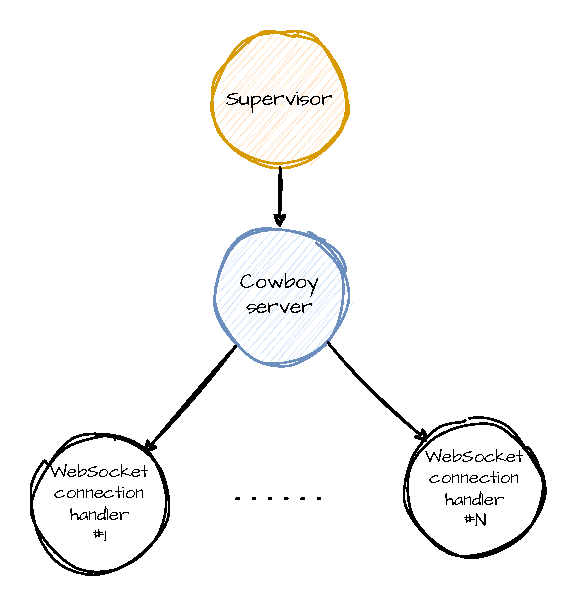
\includegraphics[width=0.5\textwidth]{img/system_architecture/erlang_diagram.pdf}
	\caption{Hierarchy of Erlang processes inside the chat server application}
	\label{fig:erlang-hierarchy}
\end{figure}


The new spawned process will call the functions belonging to the \texttt{chatroom\_websocket} module:
\begin{itemize}
    \item \texttt{init/1}: called whenever a request is received, in order to establish a websocket connection.
    \item \texttt{websocket\_handle/2}: called whenever a text, binary, ping or pong frame arrives from the client. It will handle the reception and deserialization of the JSON objects coming from the client.
    \item \texttt{websocket\_info/2}: called whenever an Erlang message arrives (i.e. a message from another Erlang process). It will forward a chatroom message to the client browser assigned to this process.
    \item \texttt{terminate/3}: called whenever the WebSocket connection is closed. It will remove its assigned user from the list of the currently online students inside the chatroom.
\end{itemize}


\subsubsection{Client-server communication}
\label{subsubsec:erlang/Client-server communication}

During the WebSocket session, all messages exchanged between the \textit{client browser} and the \textit{Cowboy WebSocket handler} are encoded in \textbf{JSON format}. Meanwhile Javascript natively supports JSON encoding/decoding inside the browser, the Erlang application requires an external dependency such as the \href{https://github.com/sile/jsone}{\textbf{jsone library}}.

The client browser can send three different kinds of JSON messages:
\begin{itemize}
    \item Request for login into a chatroom
    \item Request for the list of the currently online students in the chatroom, i.e. the students currently logged in the chatroom
    \item Chat message
\end{itemize}

The Javascript client encodes these message in the following format:
\begin{Verbatim}[samepage=true]
{
    opcode: "LOGIN",
    course: <id of the course owning the chatroom>,
    username: <username of the current user>
}

{
    opcode: "GET_ONLINE_USERS"
}

{
    opcode: "MESSAGE",
    text: <text of message>
}
\end{Verbatim}

On the other hand, the Cowboy server can send back two different kinds of JSON messages:
\begin{itemize}
    \item Current list of the currently online students in the chatroom
    \item Chat message
\end{itemize}

The encoded format is the following:
\begin{Verbatim}[samepage=true]
{
    opcode: "MESSAGE",
    sender: <sender's username>,
    text: <text of message>
}

{
    opcode: "GET_ONLINE_USERS",
    list: <list of currently online users>
}
\end{Verbatim}

\end{sloppypar}


\subsubsection{Modules overview}
The \texttt{chat\_server} application is composed of six modules:
\begin{itemize}
    \item \texttt{chat\_server\_app}: the first executed module. It starts the mnesia application and spawns the supervisor process. It implements the \texttt{application} behavior.
    
    \item \texttt{chat\_server\_sup}: the \texttt{supervisor} callback module. It's responsible to spawn a process which will handle the lifecycle of the process running the Cowboy server. It implements the \texttt{supervisor} behavior.
    
    \item \texttt{cowboy\_listener}: a \texttt{gen\_server} callback module which will start a Cowboy instance listening at port 8300 for TCP connections. It will also cleanup the Mnesia database by removing all the users assigned to this Erlang node which remained after an unexpected crash of the server.
    
    \item \texttt{chatroom\_websocket}: callback module for the module \texttt{cowboy\_websocket}. For more details see section \vref{subsubsec:erlang/overview}.
    \item \texttt{chatroom\_server}: module which implements the business logic for the WebSocket handlers.
    
    \item \texttt{mnesia\_manager}: module which offers methods to access the Mnesia database. For more details see section \vref{subsec:erlang-mnesia}. 
\end{itemize}




\subsection{Mnesia Database}
\label{subsec:erlang-mnesia}
Mnesia is a true \textbf{distributed DBMS} that we used to store chatrooms informations in a table.\\
These informations were \textbf{distributed over all the erlang nodes}, using \textit{ram\_copies} as a \textbf{storage option}.\\
How explained in the \textbf{Mnesia documentation}, the \textit{ram\_copies} storage option allows us to specify a list of nodes where this table is supposed to have \textbf{RAM copies}. A table replica of type \textit{ram\_copies} is \textbf{not written to disc} on a per transaction basis.\\
A \textbf{table with the cluster schema} of the Erlang nodes, however, \textbf{is stored on the disk} of the master node, this schema will be used by the master to identify the cluster nodes on which to run the distributed Mnesia DB.\\

As previously anticipated, there is \textbf{only one table in the database}, \textbf{\textit{online\_students}}, whose type is bag.\\
The attributes of this table are \textit{course\_id, student\_pid, student\_name} and \textit{hostname}. course\_id is the key of this table.\\
The data in this table is used to \textbf{keep track}, for each course, of all \textbf{students that join the chatrooms}.\\
\textbf{Through the use of different queries}, on this table, it is possible to retrieve the online student at any given time in order to send them messages and it is also possible to handle other needs to better manage the chatrooms behavior. \\

More in detail, the queries we implemented are:
\begin{itemize}
    \item \textit{join\_course}, which \textbf{adds a student} to a course chatroom;
    \item \textit{get\_online\_pid}, which returns the pids of students currently online in a chatroom, which is a particularly useful query for figuring out \textbf{to which erlang processes forward messages};
    \item \textit{get\_online\_students}, which \textbf{returns the usernames of students currently online in a chatroom}, these usernames will then be returned to the client in order to show the online students;
    \item \textit{logout}, which \textbf{removes a student} from the related course chatroom;
    \item \textit{remove\_logged\_students\_by\_hostname},  that \textbf{recursively removes all users} in each chatroom, \textbf{from a given node}.\\
    In fact, this last query allows us to \textbf{ guarantee a state of eventual consistency after a node crash}, which would \textbf{otherwise introduce duplicates when it is restarted}.
\end{itemize}




\subsection{Client-side: Javascript WebSocket}
As we anticipated in the section \vref{subsubsec:erlang/Client-server communication}. there is a message exchange between the browser client and the cowboy websocket handler.\\
The browser client sends and receives messages via a \textbf{websocket} that is implemented through \textbf{Javascipt}.\\
This websocket was created by using the \textbf{WebSocket API}, which provides methods and events to handle websocket connections.\\
We matched these methods and events with functions that handled them and included additional functions to make the chatroom work properly.\\

The functions that invoke the \textbf{creation and closure of the websocket} are:
\begin{itemize}
    \item \textit{connect(\_logged\_user, \_course)}, which is responsible for \textbf{creating the websocket and associating each method with the function that handles it}. This function is \textbf{called with the onload} of the body of the corresponding html page;
    \item \textit{disconnect()}, which is responsible for \textbf{invoking the websocket connection closure} and the function that handles the latter. This function is \textbf{called with the onunload} of the body of the corresponding html page. \\
\end{itemize}

The functions that \textbf{handle the websocket connection} are:
\begin{itemize}
    \item \textit{openWebsocketConnection()}, it \textbf{starts the connection with websocket}, sending the login message and also call of the refreshWebsocketConnection() function;
    \item  \textit{closeWebsocketConnection()}, is invoked when the \textbf{connection with the websocket is closed} and also call of the stopRefreshWebsocketConnection(). In addition This function tries to create a new websocket connection \textbf{in case the previous connection is involuntarily closed}, for example, after the Erlang Node, to which it was connected, \textbf{crashes};
    \item  \textit{refreshWebsocketConnection()}, it executes an \textbf{automatic refresh of the websocket connection} every 10 sec by sending GET\_ONLINE\_USERS message through the websocket connection;
    \item \textit{stopRefreshWebsocketConnection()}, it \textbf{stops the automatic refresh of the websocket connection};
    \item \textit{sendObjectThroughWebsocket(isWebsocketConfigurationMessage, ...args)},\\ it \textbf{creates and sends a JSON object} through the websocket connection;
    \item \textit{receiveObjectThroughWebsocket(event)}, it \textbf{handles the receive event of a JSON object}, parse it and executes the action provided by the opcode parameter of the object;
    \item \textit{handleWebsocketError()}, it \textbf{handles the possible errors} with the websocket connection.
\end{itemize}


\subsection{Master node}
In order to correctly configure the Mnesia database and launch the remote Erlang nodes , we developed a \textit{master application} which executes the following operations:
\begin{itemize}
    \item It connects to the remote nodes by means of \texttt{net\_kernel:connect\_node/1}.
    
    \item It starts its local Mnesia process, creates a persistent schema with the other Erlang nodes (if it doesn't already exist) and creates the \textit{online\_students} table inside the schema (if it doesn't already exist). The new table only resides on the chat\_server nodes.
    
    \item It spawns the chat\_server application processes on the remote nodes.
\end{itemize}

The master application process runs on the same node as the Nginx load balancer.



\subsection{Load balancer}
In order to fairly distribute the load relative to the chatroom and fully exploits the benefits deriving from a distributed Erlang deploy (such as high availability, fault tolerance, scalability...), a \textit{load balancer} has been deployed on node \texttt{10.2.1.4}.

We chose \textbf{Nginx} for this purpose since it natively supports the WebSocket protocol both as \textbf{reverse proxy} and \textbf{load balancer}, so it's a perfect match for our requirements.

The Nginx server has been configured to listens on port 8300 and to proxy every WebSocket connection to one of the remote chat\_server nodes.

\begin{verbatim}
worker_processes 1;
worker_rlimit_nofile 8192;

events {
  worker_connections  1024;
}

http {
    map $http_upgrade $connection_upgrade {
        default upgrade;
        '' close;
    }
	
    upstream websocket {
        server 10.2.1.52:8300;
        server 10.2.1.31:8300;
        server 10.2.1.51:8300;
    }
	
    server {
        listen 8300;
        location / {
            proxy_pass http://websocket;
            proxy_http_version 1.1;
            proxy_set_header Upgrade $http_upgrade;
            proxy_set_header Connection $connection_upgrade;
            proxy_set_header Host $host;
        }
    }
}
\end{verbatim}




%% GLASSFISH
\section{Glassfish}
\begin{figure}[H]
    \centering
     \includegraphics[width=1\textwidth]{img/system_architecture/system_architecture.png}
    \caption{\label{fig:system_architecture} System Architecture Schema.}
\end{figure}

The web application, as we can see in figure \ref{fig:system_architecture}, consists of a \textbf{Client Application}, a \textbf{Jakarta Application Server}, and \textbf{multiple erlang servers}.\\
The Jakarta EE Application Server, which implements most of the functionality of the application, uses as its reference implementation, \textbf{Glassfish 6.2.5} and also communicates with a \textbf{MySql relational database} located on a different machine.\\
The Erlang Servers, which are managed by a \textbf{Load Balancer} on another machine, handle the Chatrooms of the application through an \textbf{HTTP websocket communication}.\\
For more specific details, all these modules will be analyzed individually.
\newpage

\subsection{Web}
In the Maven project \textbf{web}, as said before, we introduced the Servlets and JSP needed. In order to separate each page and keep the logic of each web page divided we implemented a Servlet for each page that will gather the data needed to build the HTML page through JSP technology. In addition, this project contains all the necessary part for displaying resources, so: CSS, JavaScript and the images, everything can be found inside the webapp/assets folder. \\
Servlets are divided in four main categories based on the type of users to which are dedicated:
\begin{itemize}
    \item Professor's servlets
    \item Student's servlets
    \item Admin's servlets
    \item Common servlets
\end{itemize}
\ \\
Each servlet, that don't belong to common category, access session information to check:
\begin{itemize}
    \item if the current user has already logged in: otherwise will redirected to login page
    \item whether the user is in the appropriate category to access that type of resource: otherwise the malicious user will be redirected to his portal page
\end{itemize}
Common servlets instead, such as login and logout, don't need these kind of techniques since there is no difference between the resource behaviour and the user category.
\ \\
In the end each servlet, upon a request, can call the methods of the EJBs that implement the related application logic obtaining their remote reference through JNDI.\\
In the table \ref{tab:servlets} there is a list of the Servlets that has been implemented.

\begin{table}[h]
\centering
\caption{Servlet List}
\label{tab:servlets}
\begin{tabular}{|c|c|c|}
\hline
\textbf{Visibility} & \textbf{Servlet Name} & \textbf{Implemented methods} \\ \hline
All & LoginServlet & POST\\ \hline
All & LogoutServlet & GET \& POST\\ \hline
Students & SignUpServlet & GET\\ \hline
Students & StudentPortalServlet & GET\\ \hline
Students & ChatroomServlet & GET\\ \hline
Students & StudentProfileServlet & GET \& POST\\ \hline
Students & StudentCourseServlet & GET \& POST\\ \hline
Students & StudentBookingServlet & GET \& POST\\ \hline
Professor & ProfessorPortalServlet & GET\\ \hline
Professor & ProfessorMeetingServlet & GET \& POST\\ \hline
Professor & ProfessorDeleteCourseServlet & GET \& POST\\ \hline
Professor & ProfessorCreateCourseServlet & GET \& POST\\ \hline
Admin & AdminCreateProfessorServlet & GET \& POST\\ \hline
Admin & AdminPortalServlet & GET\\ \hline
Admin & AdminUserManagementServlet & GET \& POST\\ \hline
\end{tabular}
\end{table}


\subsection{Ejb-Interfaces}
In the \textbf{ejb-interfaces} Maven project, as said before, there are \textbf{all the interfaces, for the calls to EJBs}. \\
These interfaces represents the \textbf{contract with the client} and they are all \textbf{\textit{remote}} interfaces. \\
In this Maven project there are also all the DTOs and the enumerates type, that will be discussed in the POJOs section.\\

The interfaces that we have implemented are:
\begin{itemize}
    \item \textbf{BookedMeetingEJB};
    \item \textbf{CourseEJB};
    \item \textbf{UserEJB}.
\end{itemize}


\subsection{Ejb}
The \textbf{ejb} Maven project, as previously introduced, contains the \textbf{implementation of the classes declared in the ejb-interfaces} with the \textbf{business logic needed} to provide the required functionalities.\\
The type of the \textbf{EJB class implementation} is \textbf{\textit{Stateless}}.\\
As we anticipated in the ejb-interfaces section, three ejb were used to implement the business logic of the application:
\begin{itemize}
    \item \textbf{BookedMeetingEJBImpl}, this EJB is the \textbf{only one where a DAO was created} for, as it provided business logic \textbf{beyond simply accessing database resources}.\\
    In fact, this EJB, in addition to retrieving data back from the database, through its DAO methods, grants us the ability to view the entire schedule of a professor's slots and perform various operations on it;
    \item \textbf{CourseEJBImpl}, This EJB allows us to \textbf{access course data}, it gives us the ability to search through course names and professors, but also to \textbf{perform all these operations applied only to the starred courses} of the specific student.\\
    We can also insert or delete courses, as well as promote or retract them from the starred status;
    \item \textbf{UserEJBImpl}, this EJB gives us the ability to manage the \textbf{business logic of the login and of the signup} of the students and their interaction with the db.
    It also provides operations that can \textbf{alter a user's status}, through banning, or operations such as \textbf{create professor and student search}.
\end{itemize}
\newpage

\subsection{POJOs: DTOs, Enums and DAOs}
\label{subsec:pojos}
In the Maven projects \textbf{ejb-interfaces} and \textbf{ejb}, we had to introduce some \textit{Plain Old Java Objects} (\textbf{POJOs}) in order to efficiently share data between EJBs and Servlets and to separate different concerns:

\begin{itemize}
    \item Package \texttt{dto} (project \textit{ejb-interfaces}): contains all the \textbf{Data Transfer Objects} (DTOs) necessary to transfer information from the business logic tier to the presentation tier. The chosen approach was to develop a separate DTO for every single information, in order to minimize the transferred data and to better separate each concern.
    
    \item Package \texttt{enums} (project \textit{ejb-interfaces}): contains the \textit{UserRole} enum class, needed to correctly identify the role of an user (student, professor, admin).
    
    \item Package \texttt{dao} (project \textit{ejb}): contains the \textbf{Data Access Object} (DAO) responsible for all the data accesses concerning the booking of meetings. The reason only one DAO has been implemented stems from the fact that BookedMeetinEJB is the only EJB that provides a business logic beyond the simple database access, by manipulating data to make the low-level implementation transparent with regards to the presentation tier. 
\end{itemize}


%% MySQL
\section{MySQL Server}

Finally, in order to ensure consistency, permanence and availability of data, MySQL server was used.
The final structure of our database can be observed in figure \ref{fig:mysql_er} and consists of the following tables:
\begin{itemize}
    \item \textbf{Admin}: Table intended to contain the information necessary to allow the admin to log in. It is not linked to any other table since there is no specific information to be maintained for this category of user 
    \item \textbf{Student}: Table intended to contain all the information needed for student login plus some personal information needed to identify the student
    \item \textbf{Professor}: Table intended to contain all the information needed for the professor's login plus some personal information needed to identify the professor
    \item \textbf{Course}: Table representing the course entity, has as foreign key the id of the professor who owns the course
    \item \textbf{Meeting\_slot}: Table intended to contain the list of weekly slots the course makes available to students. The only foreign key is used to identify the course that has made that slot available
    \item \textbf{Booked\_meeting}: Table intended to contain the list of slots booked by a student. It has two foreign keys, one needed to identify the student who booked that meeting and the other that binds the meeting to the slot of the course
    \item \textbf{Student\_starred\_course}: Table needed to keep in memory the set of courses that each student has added to favorites. It has two foreign keys, the combination of which constitutes the primary key, corresponding to the id of the student who added the course to the favorites and the id of the course 
\end{itemize}
\ \\
\begin{figure}[ht]
	\centering
	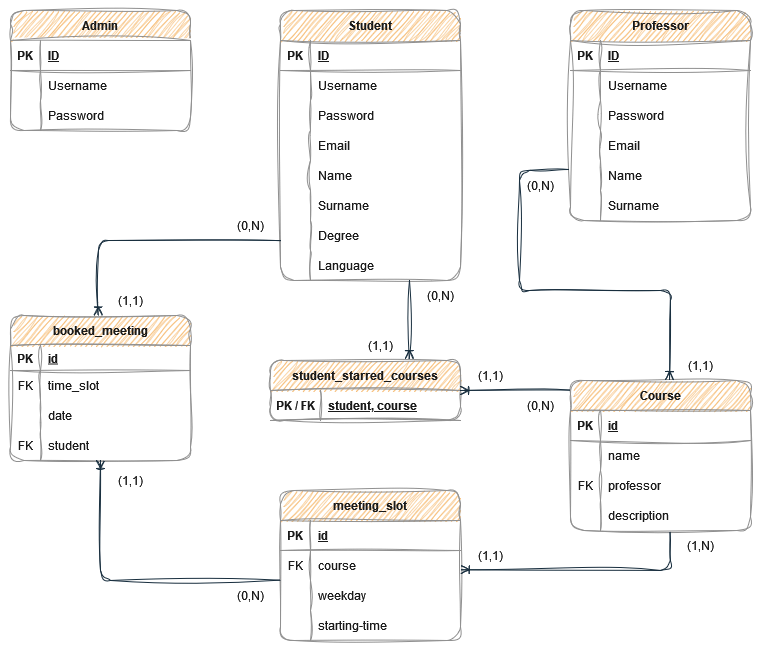
\includegraphics[width=0.8\textwidth]{img/mysql/er.png}
	\caption{Entity-Relation diagram of MySQL DB}
	\label{fig:mysql_er}
\end{figure}

    \chapter{User Manual}

% LOGIN PAGE
\section{Login page}
The root page of the webapp allows a user to login into the platform, by enterin their username, password and role (student, professor or admin).

It's also available a button for unregistered students which redirects them to the sign-up page.

\begin{figure}[H]
    \centering
    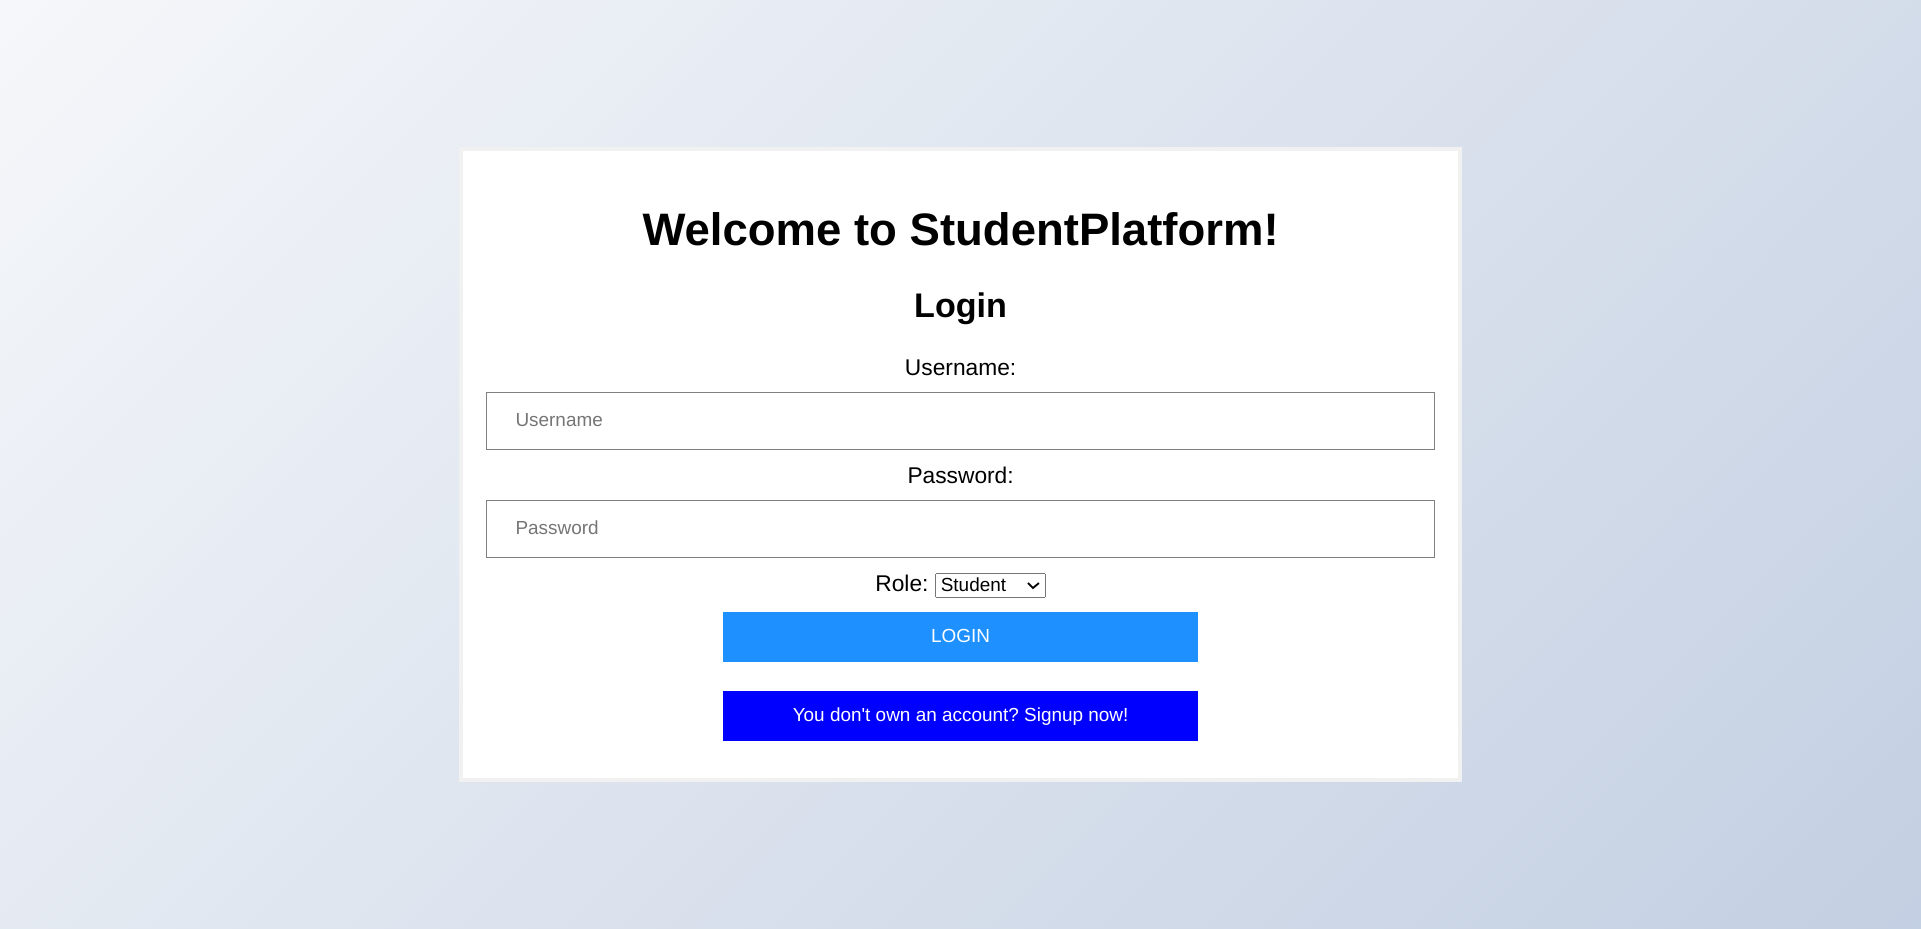
\includegraphics[width=\textwidth]{img/user_manual/index.png}
    \caption{Screenshot of login page}
\end{figure}

\newpage

% SIGN-UP PAGE
\section{Sign-up page}
This page allow unregistered users to sign up to the platform.\\
It can be accessed from login page and shows a list of fields that the user is required to fill with its personal information in order to sign up.
There are two buttons at the bottom of the page: the first allows the user to sign up for the platform, the second allows the user to return to the login page. \\
After that the first button has been clicked if the sign-up operation has been successful the user will get redirected to login page, otherwise an error message will appear.

\begin{figure}[H]
    \centering
    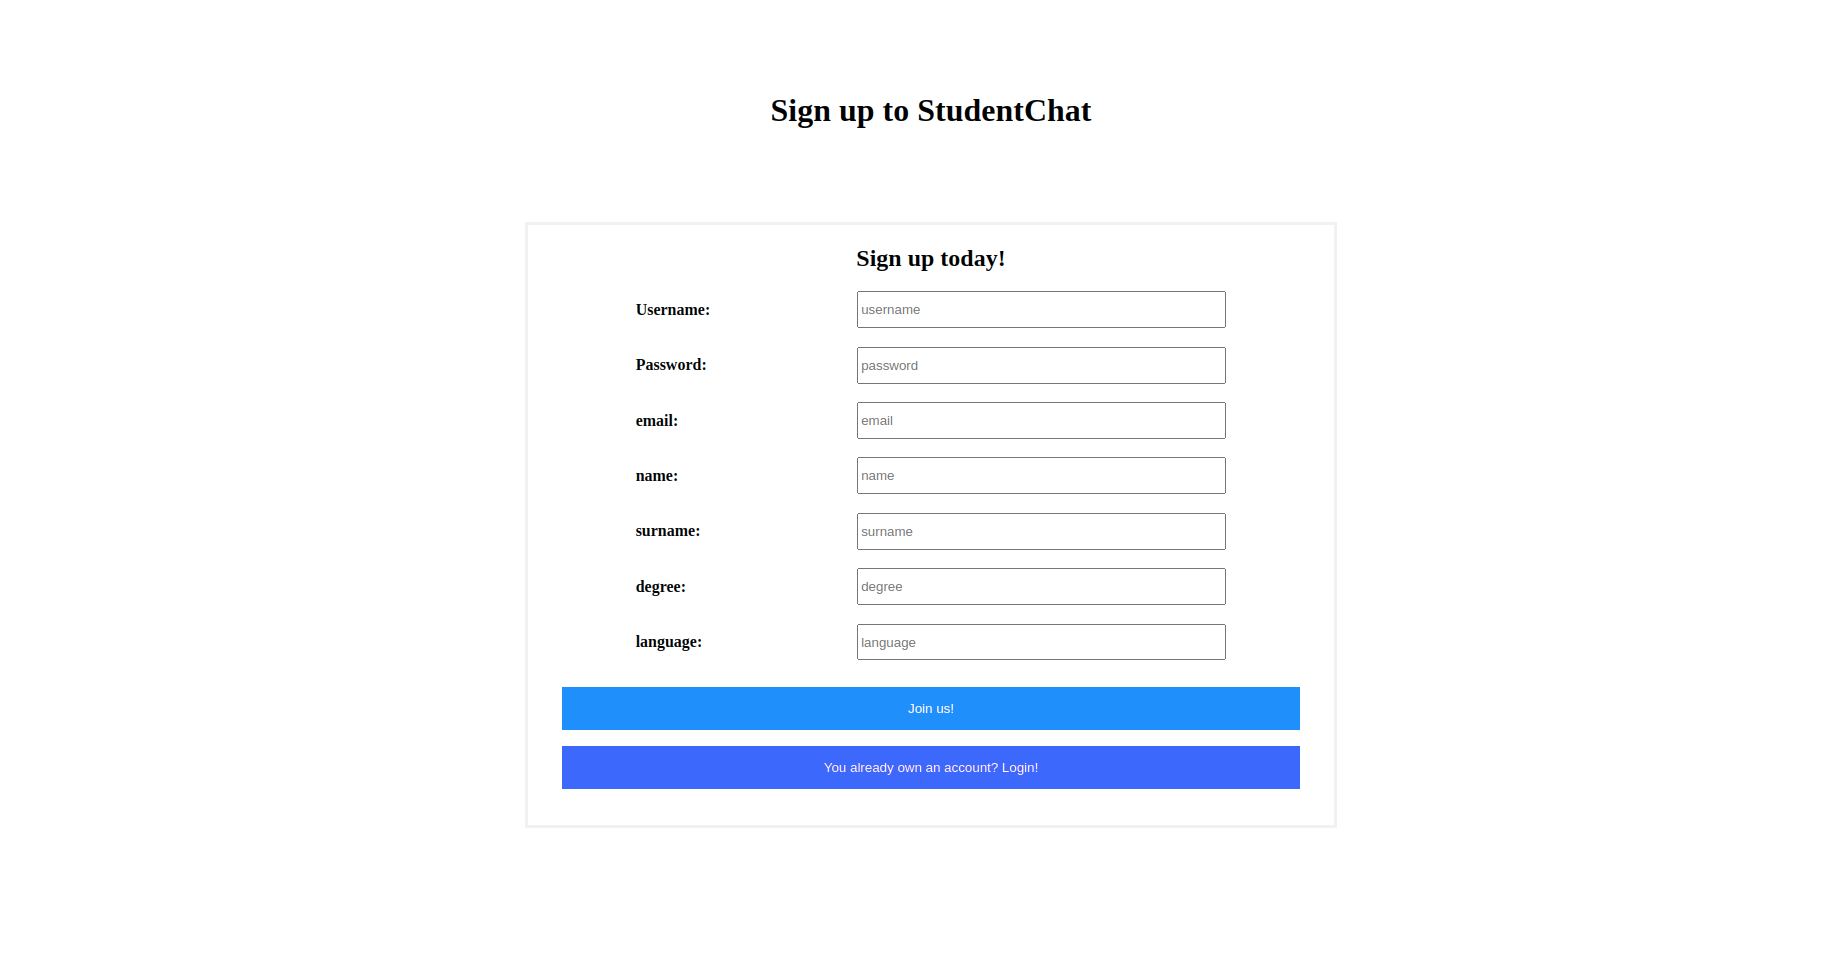
\includegraphics[width=\textwidth]{img/user_manual/student/signup.png}
    \caption{Screenshot of sign-up page}
\end{figure}
\newpage

% STUDENT SECTION
\section{Student section}

\subsection{Portal Page}
This page shows the student portal.\\

The portal displays all the courses that are on the platform.\\
The student can search for the courses he is interested in, using the research bar, searching by course name or by professor's last name.\\
He can also view only the courses he has marked as starred.\\
To access a course, simply click on the blue box of the chosen course.\\

\begin{figure}[H]
    \centering
     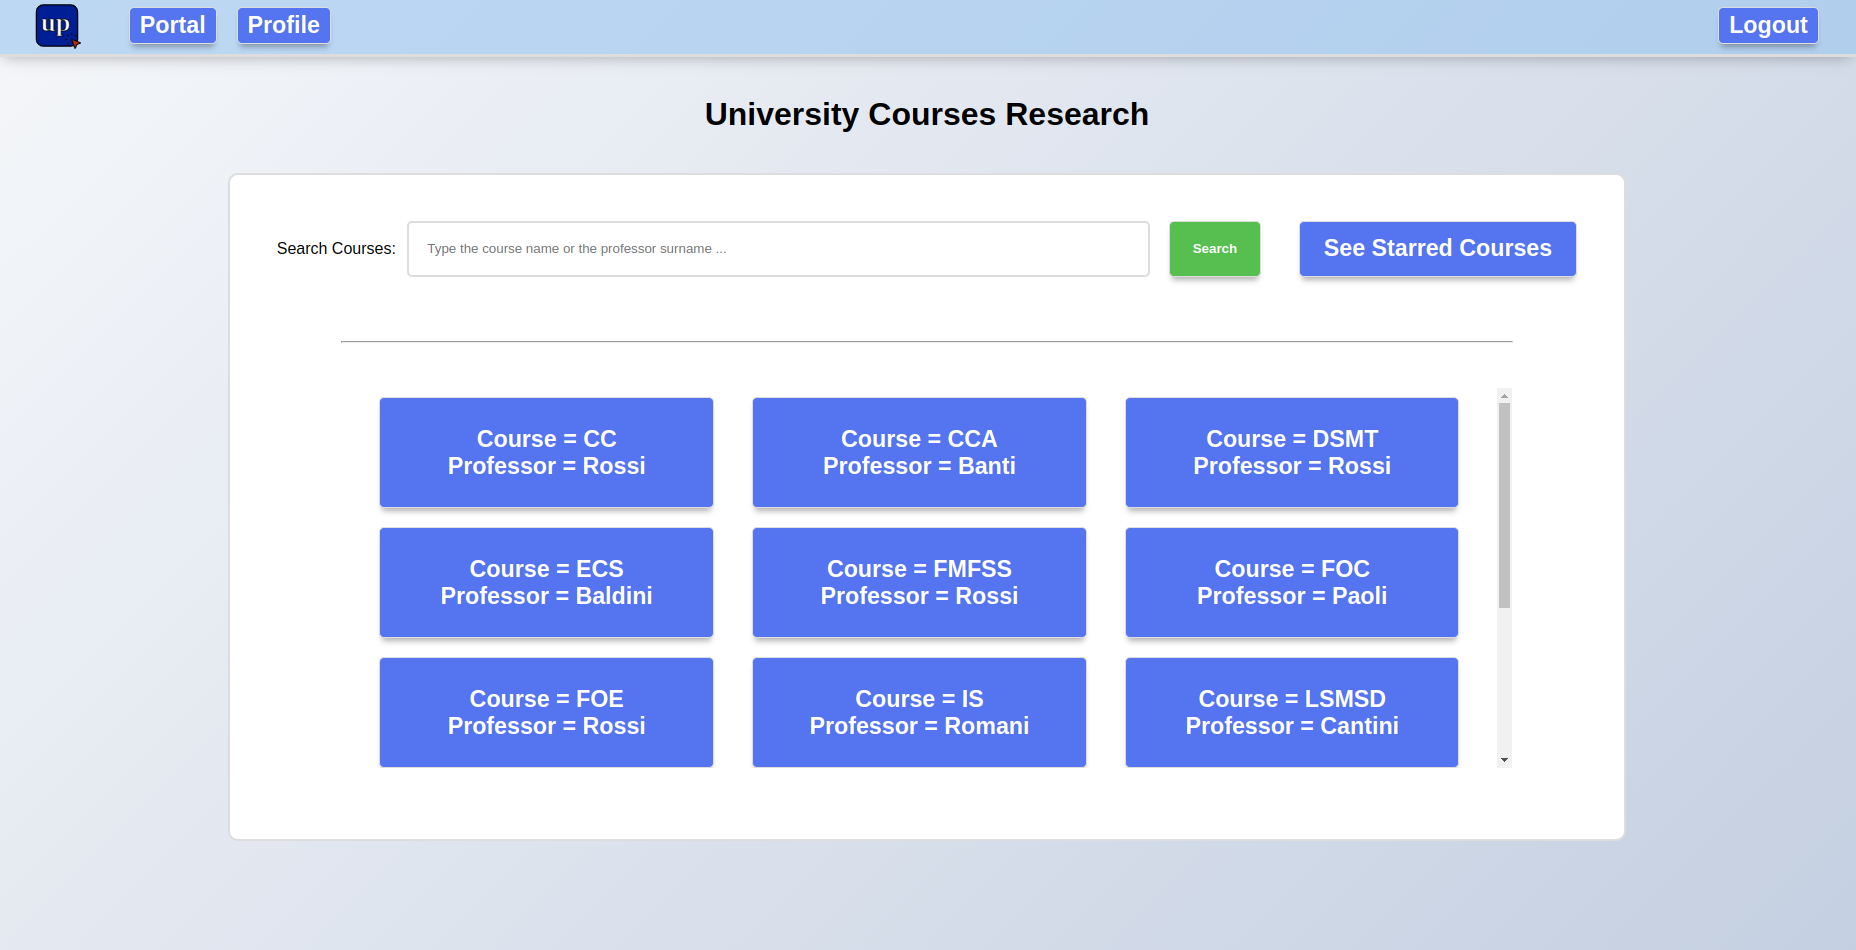
\includegraphics[width=1\textwidth]{img/user_manual/student/student-portal.png}
    \caption{\label{fig:student-portal} Screenshot of the student's portal.}
\end{figure}

As we can see from the figure, there is a topbar at the top of the page, this topbar is also present in all the other student pages.\\
Through this topbar we can return to this page, view the student's profile or log out.
\newpage

\subsection{Course page}
This page shows the details of a course.

It also provides buttons to access the corresponding chatroom and book a meeting with the professor.

\begin{figure}[H]
    \centering
    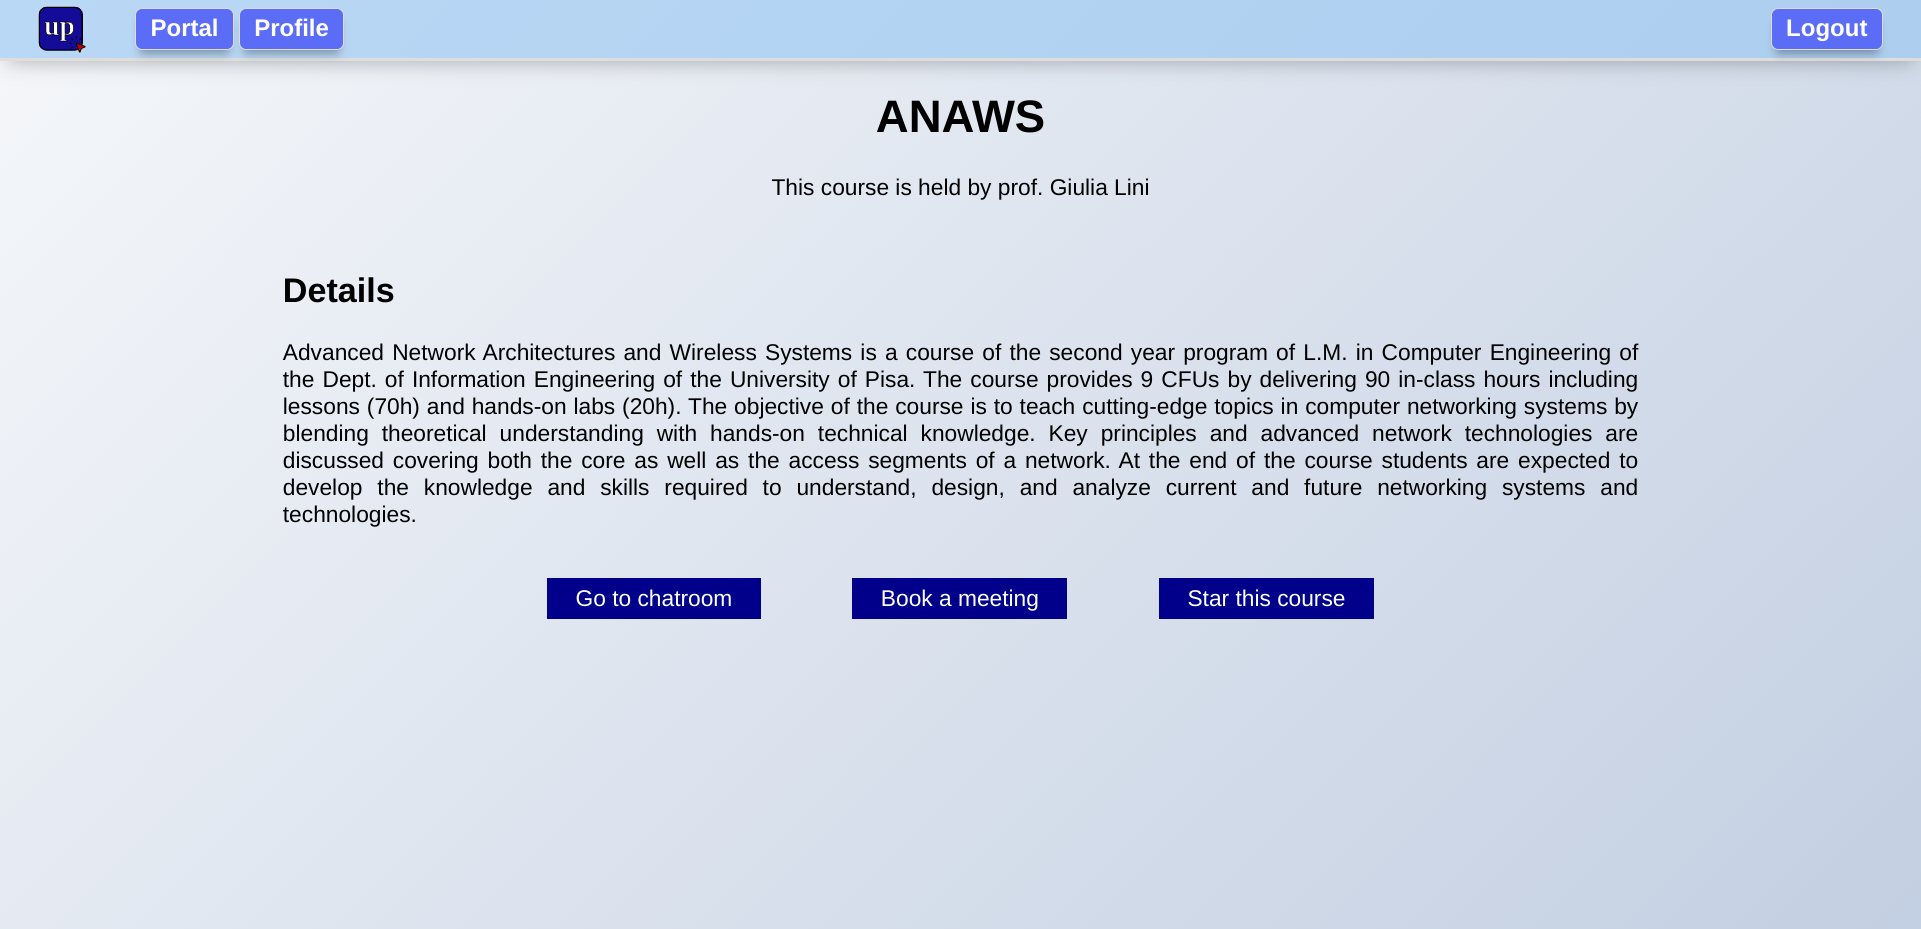
\includegraphics[width=\textwidth]{img/user_manual/student/student-course-1.png}
    \caption{Screenshot of a course page}
\end{figure}

Moreover, it is possible for a student to star the course, so that it can be shown in a separate section on their own portal page. When a student clicks on the button \textit{Start this course}, an alert pop-up spawns to notify the success of the request. The same pattern applies for the removal of a star (\textit{unstar}).

\begin{figure}[H]
    \centering
    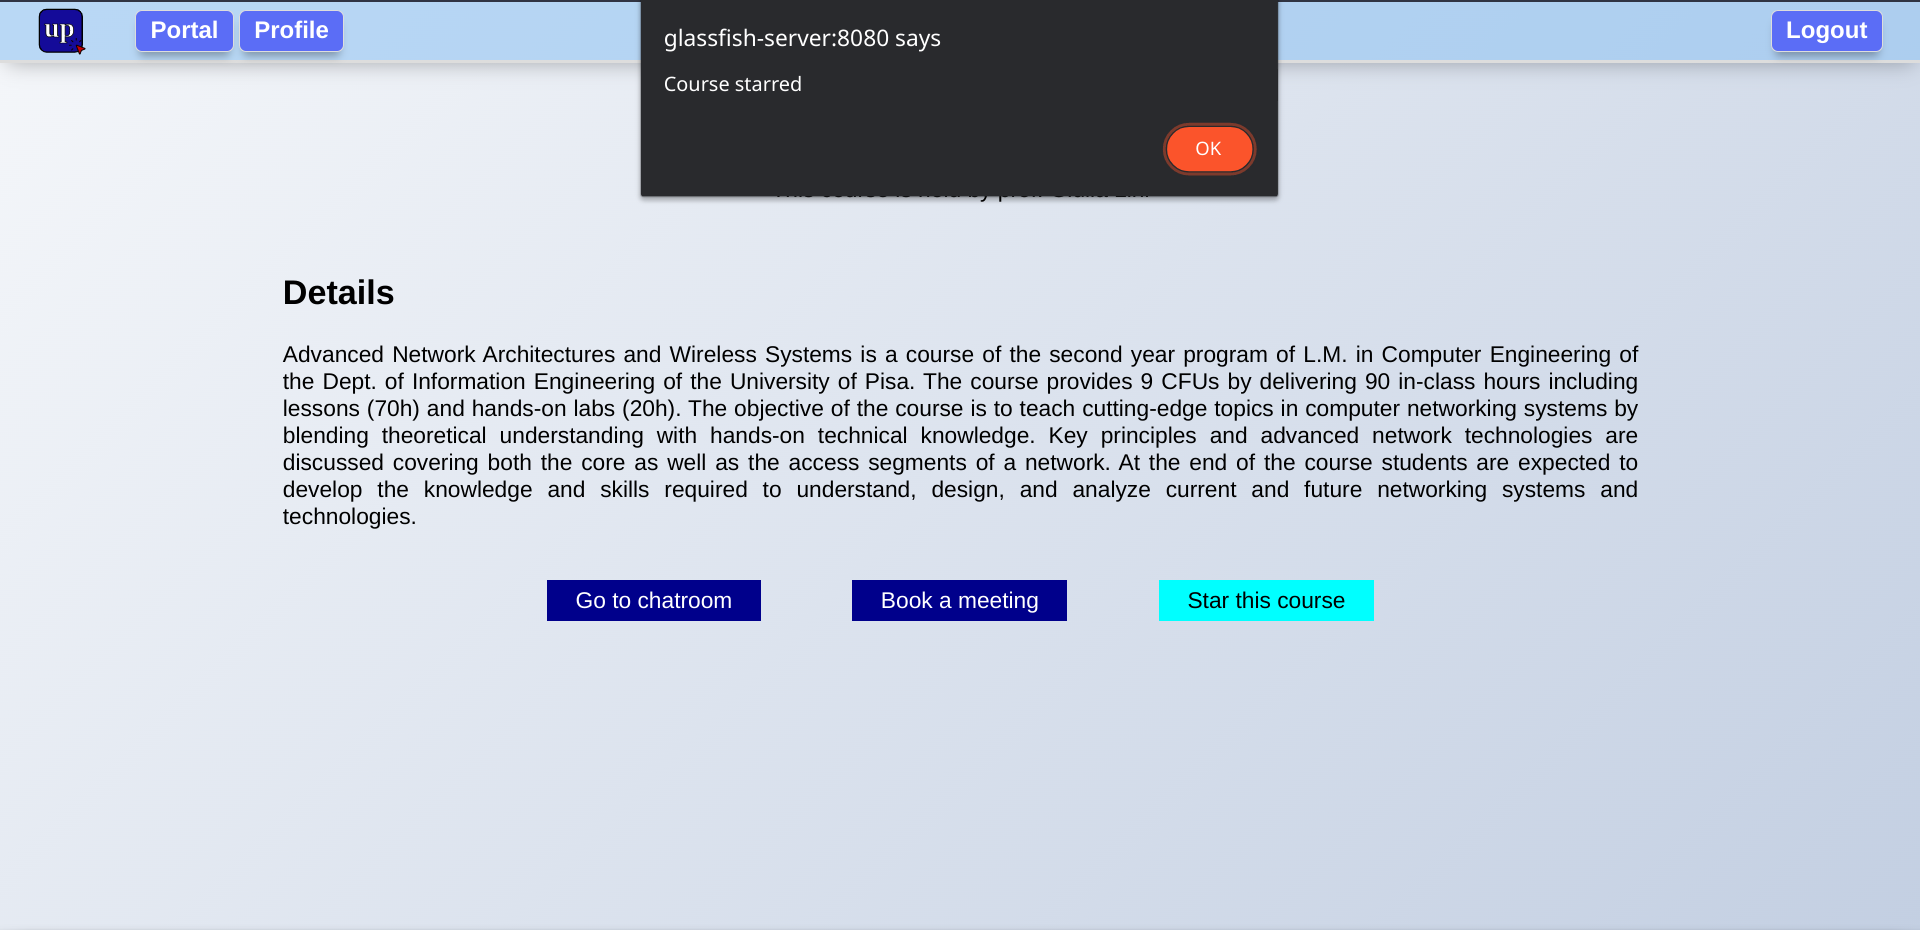
\includegraphics[width=\textwidth]{img/user_manual/student/student-course-2.png}
    \caption{Screenshot of a course page showing the alert pop-up which notify that \textit{the course has been successfully starred}}
\end{figure}

\newpage

\subsection{Chatroom page}
This is the chatroom page for a specific course.\\
On this page it is possible to chat with other students who are connected to the same chatroom of the same course.\\
A student can:
\begin{itemize}
    \item View the students currently online in the chatroom;
    \item Send messages in the chatroom through the provided input field;
    \item View messages sent by other students.
\end{itemize}

\begin{figure}[H]
    \centering
     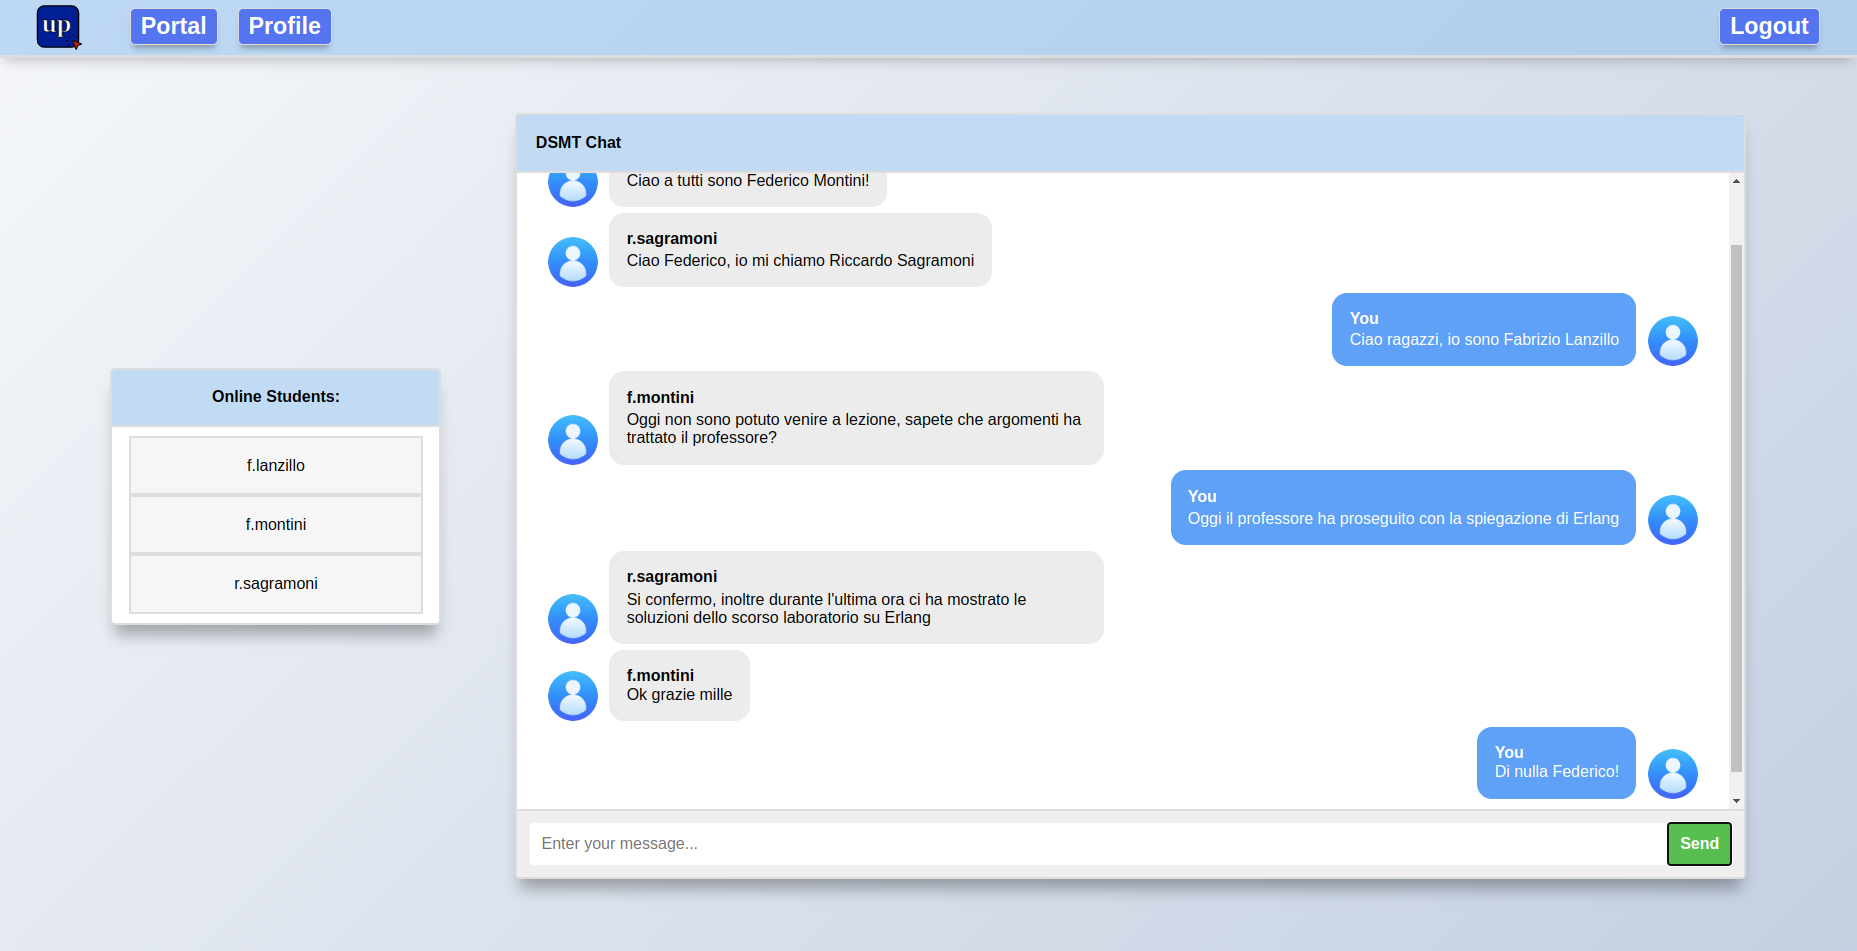
\includegraphics[width=1\textwidth]{img/user_manual/student/chatroom.png}
    \caption{\label{fig:student-chatroom} Screenshot of the student chatroom page.}
\end{figure}
\newpage

\subsection{Booking page}
The page shows the slots in which the student can book a meeting with the course's professor.\\
The student, in this page, can both book a meeting clicking on the chosen slot or switch month in which he wants to book. 
\begin{figure}[H]
    \centering
    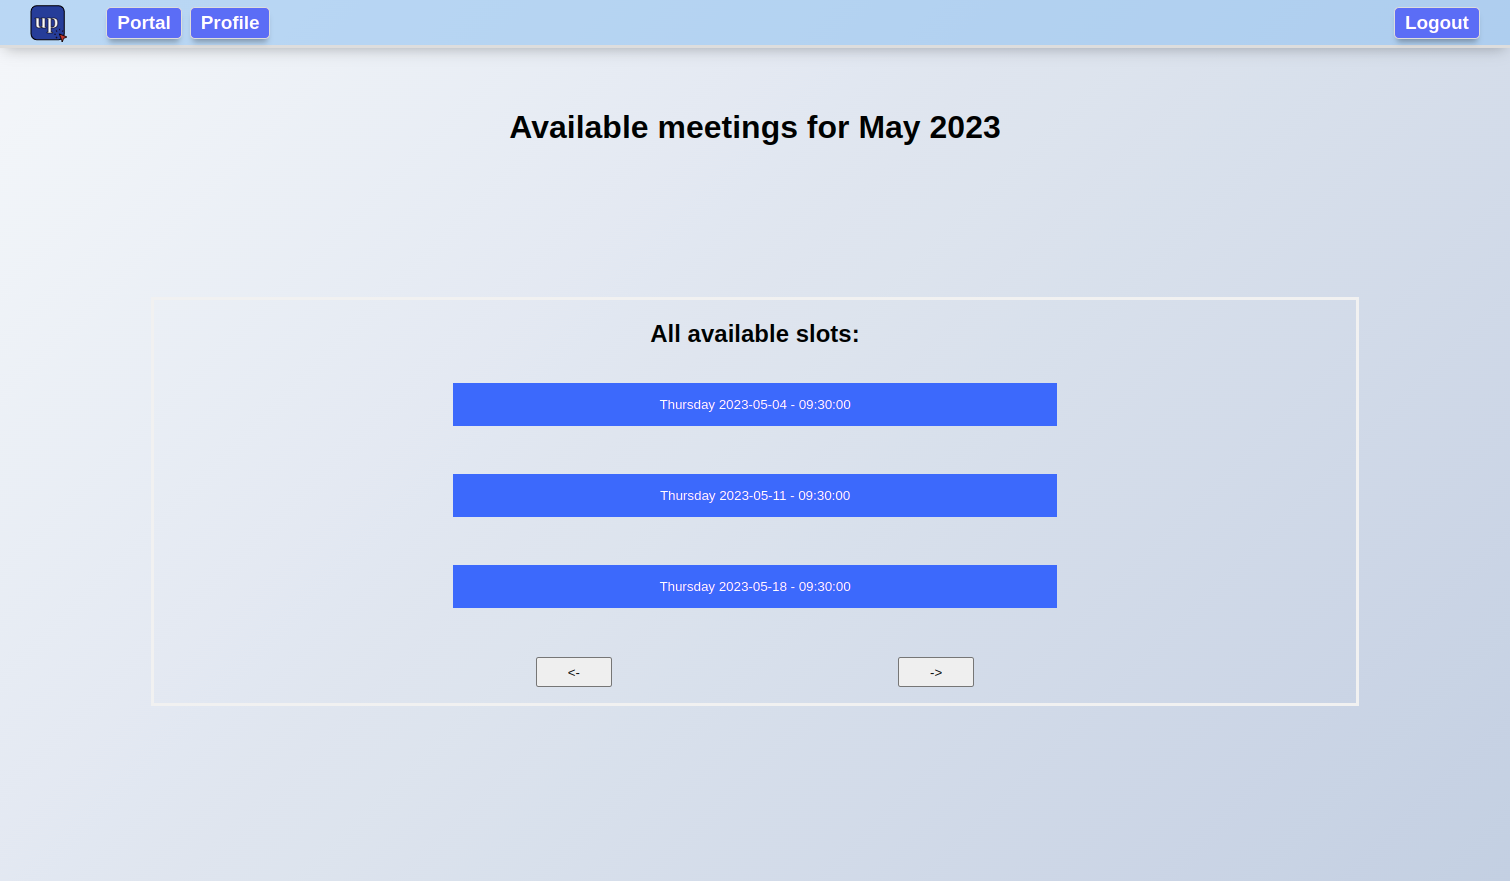
\includegraphics[width=\textwidth]{img/user_manual/student/booking.png}
    \caption{Screenshot of student/booking page}
\end{figure}

Booking a slot the pages shows a message stating the result of the operation.
\begin{figure}[H]
    \centering
    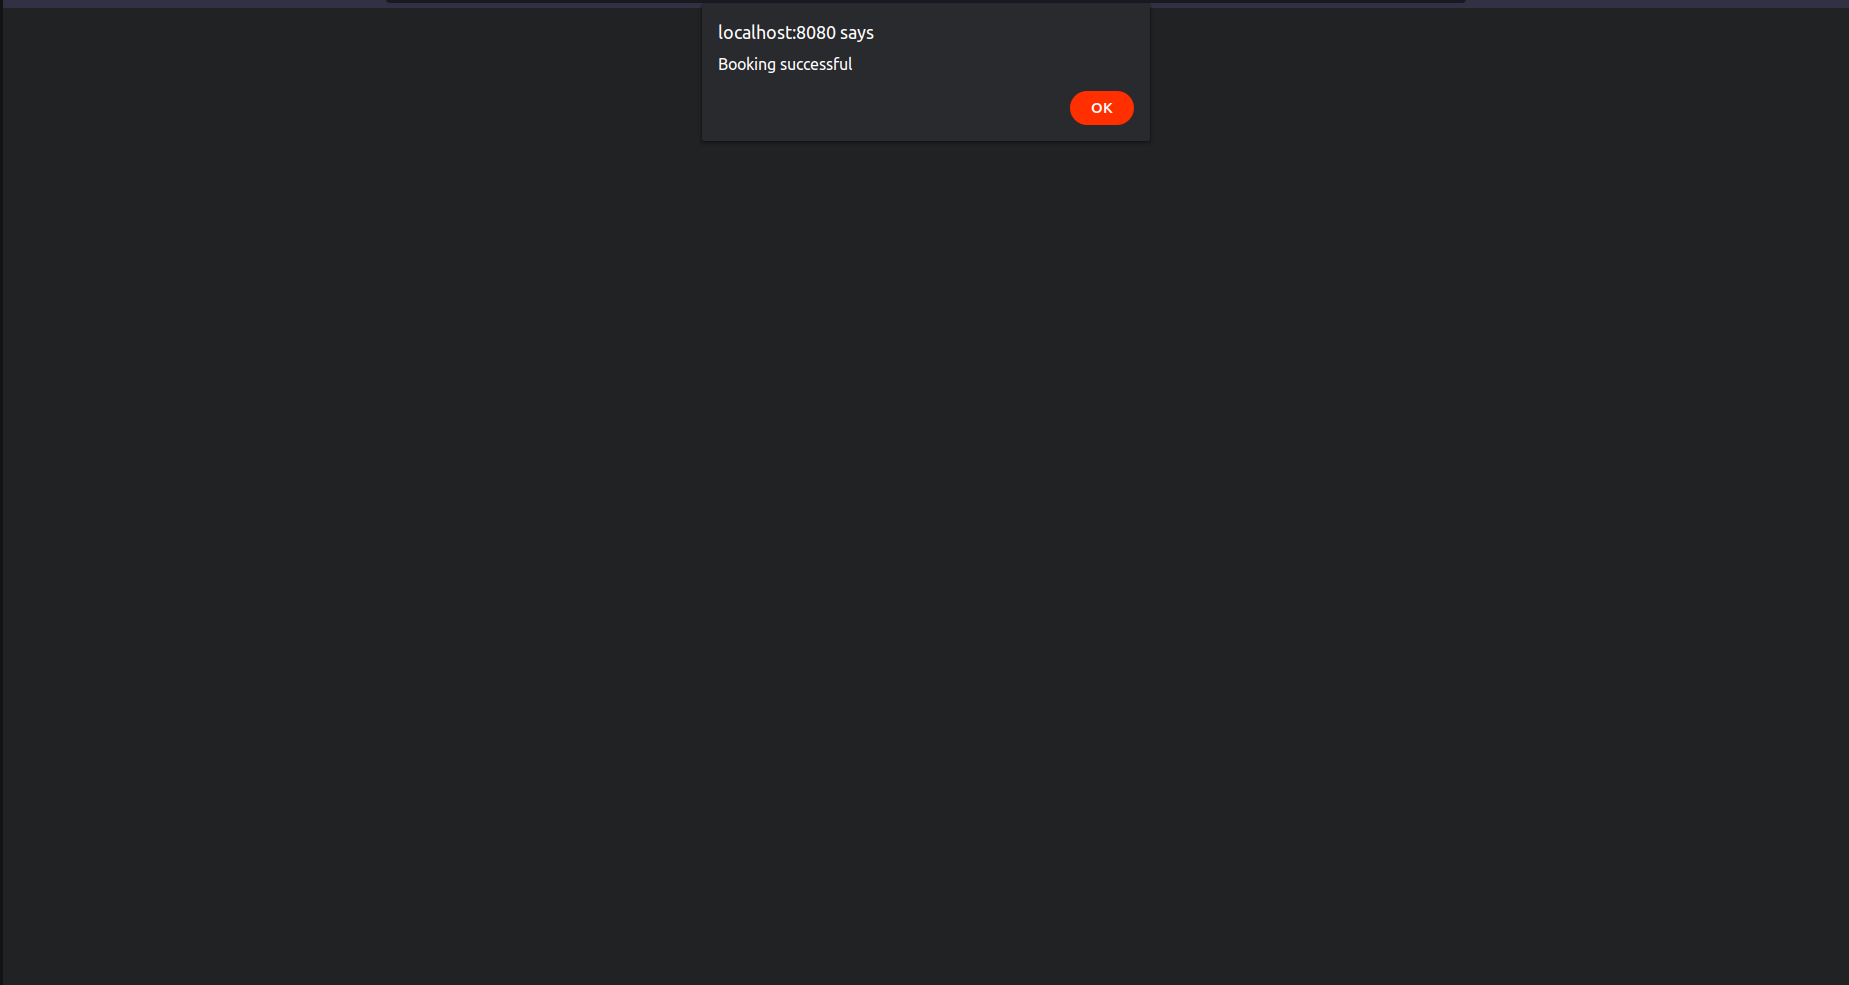
\includegraphics[width=\textwidth]{img/user_manual/student/booking-response.png}
    \caption{Screenshot of booking response}
\end{figure}
\newpage

\subsection{Profile Page} 
This is the student profile page, accessible only from the topbar.\\
Here the student can view all his/her meetings that he/she has booked.\\
If the student wishes to delete a meeting, simply click on the blue box of the corresponding meeting.\\

\begin{figure}[H]
    \centering
     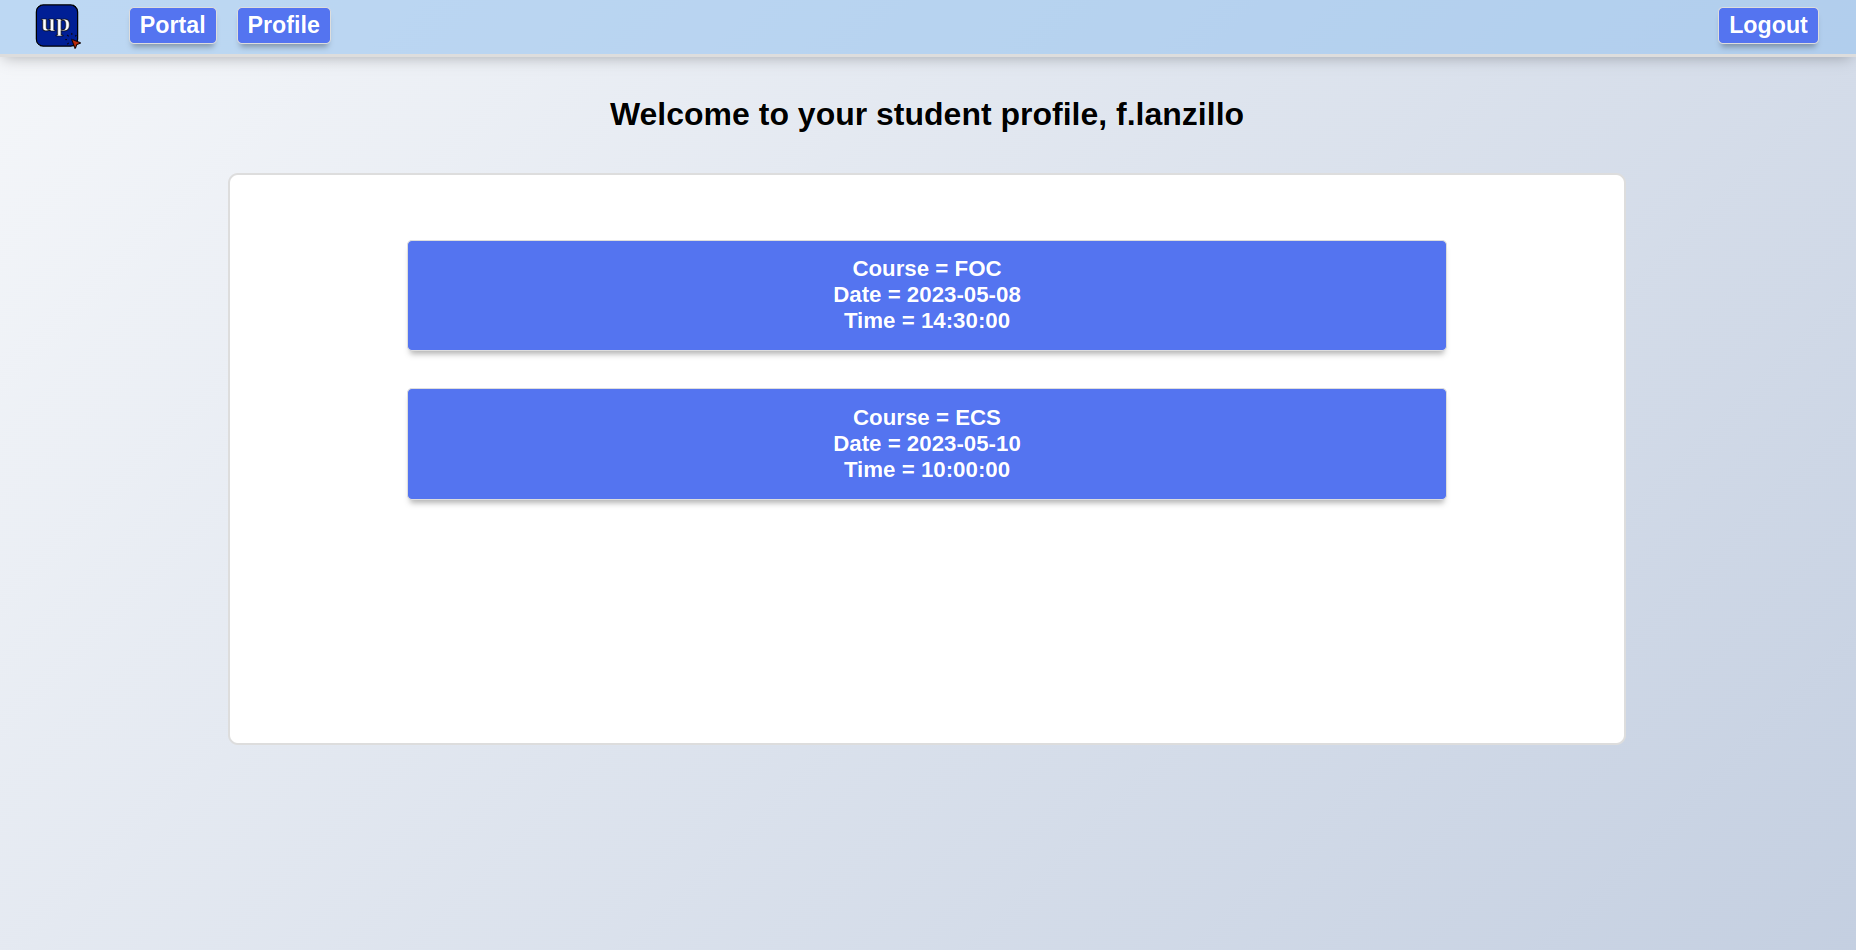
\includegraphics[width=0.95\textwidth]{img/user_manual/student/profile.png}
    \caption{\label{fig:student-profile-1} Screenshot of the student profile page.}
\end{figure}

Immediately after selecting the meeting to be deleted, an alert pops up and asks for the confirmation for the delete.\\
If the student wants to confirm he/she must click on the delete button otherwise on the x.\\

\begin{figure}[H]
    \centering
     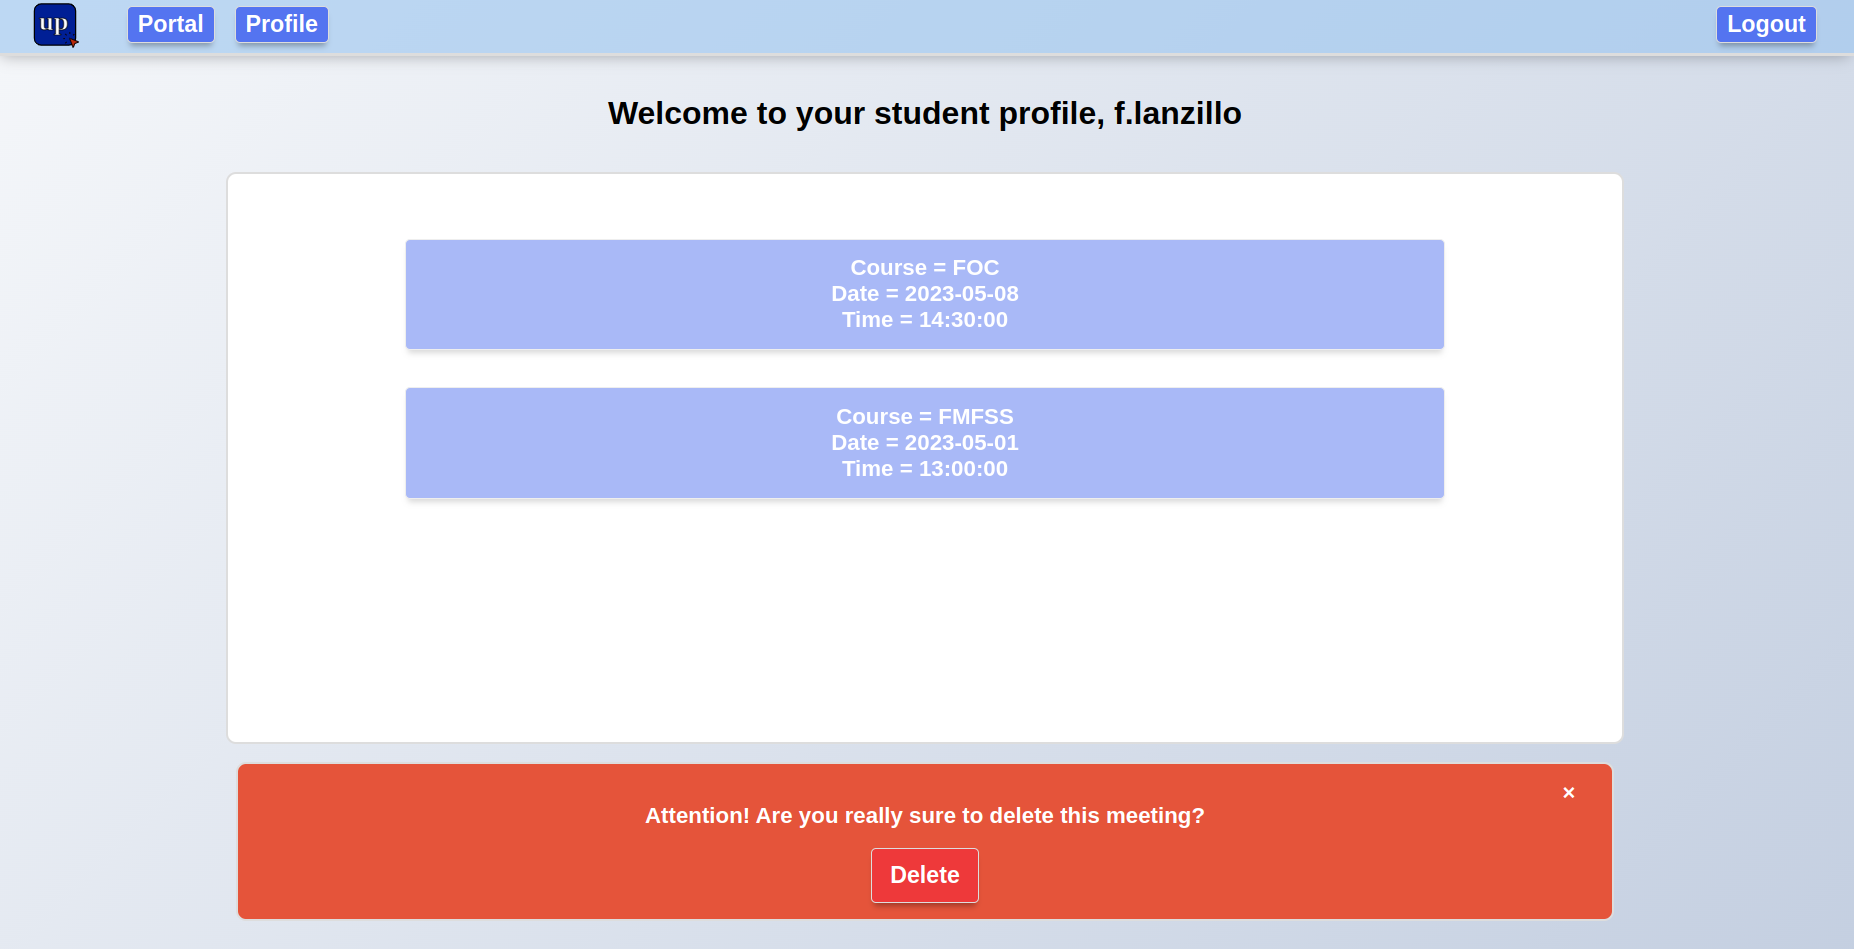
\includegraphics[width=0.95\textwidth]{img/user_manual/student/profile-delete-alert.png}
    \caption{\label{fig:student-profile-2} Screenshot of the delete alert of the student profile page.}
\end{figure}

The page shows a message with the result of the delete operation.\\

\begin{figure}[H]
    \centering
     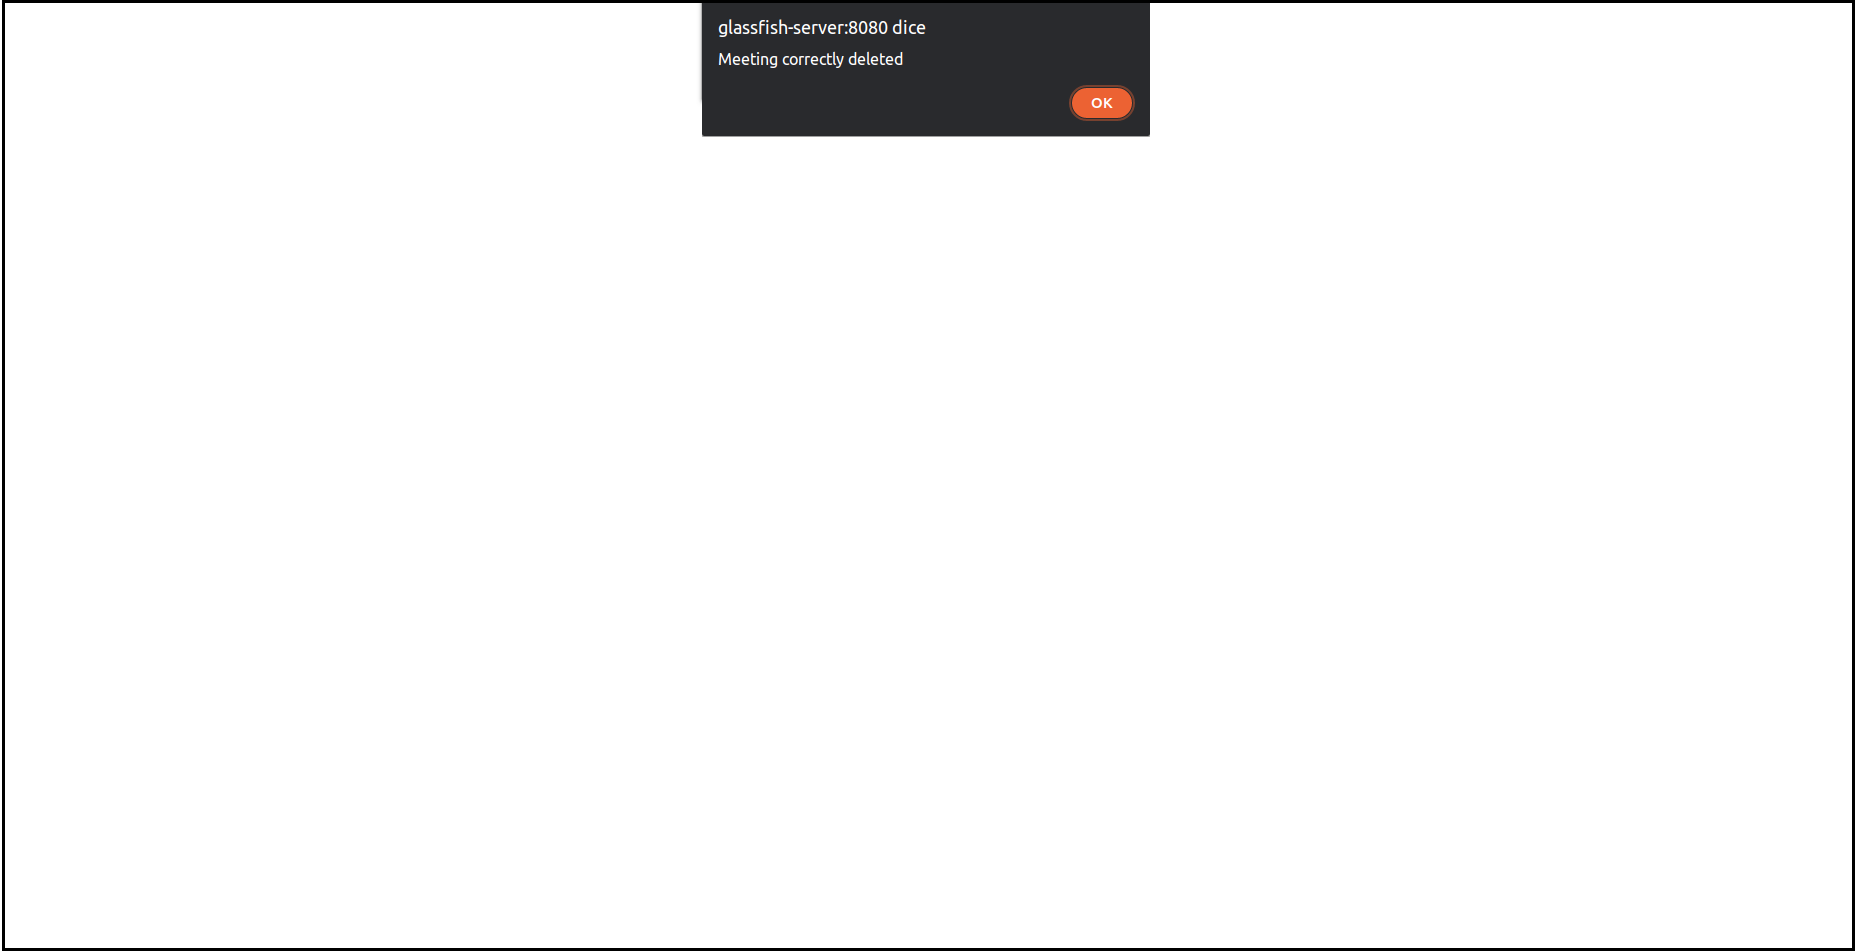
\includegraphics[width=1\textwidth]{img/user_manual/student/profile-alert.png}
    \caption{\label{fig:student-profile-3} Screenshot of the student profile page after the successful delete of the meeting.}
\end{figure}
\newpage

% PROFESSOR SECTION
\section{Professor section}

\subsection{Portal page}
The portal page for professors provides buttons for the three main operations allowed to professors:
\begin{itemize}
    \item Creating a course.
    \item Deleting a course belonging to them.
    \item Checking all their upcoming scheduled meetings with students.
\end{itemize}

\begin{figure}[H]
    \centering
    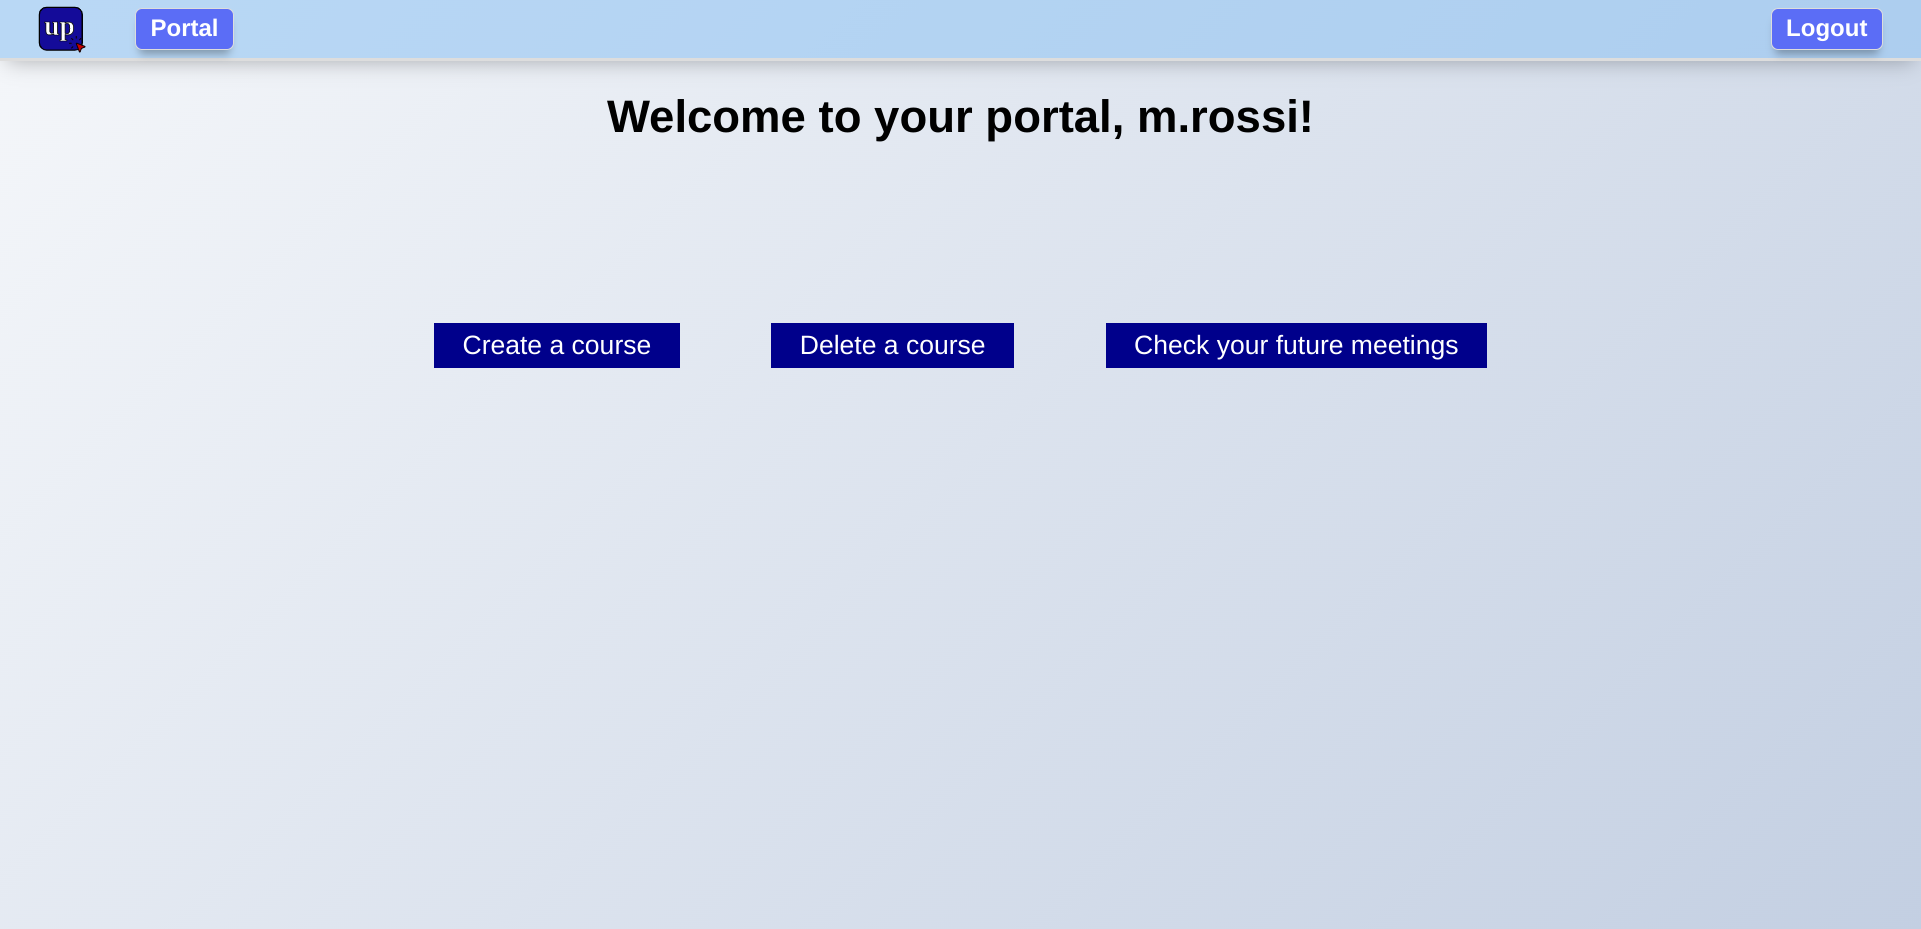
\includegraphics[width=\textwidth]{img/user_manual/professor/professor-portal.png}
    \caption{Screenshot of the professor's portal}
\end{figure}

\newpage

\subsection{Create a course}
This page provides a form to create a new course.
Professors can enter the course name and details, and they can specify the weekly time slots for meeting with students.

\begin{figure}[H]
    \centering
    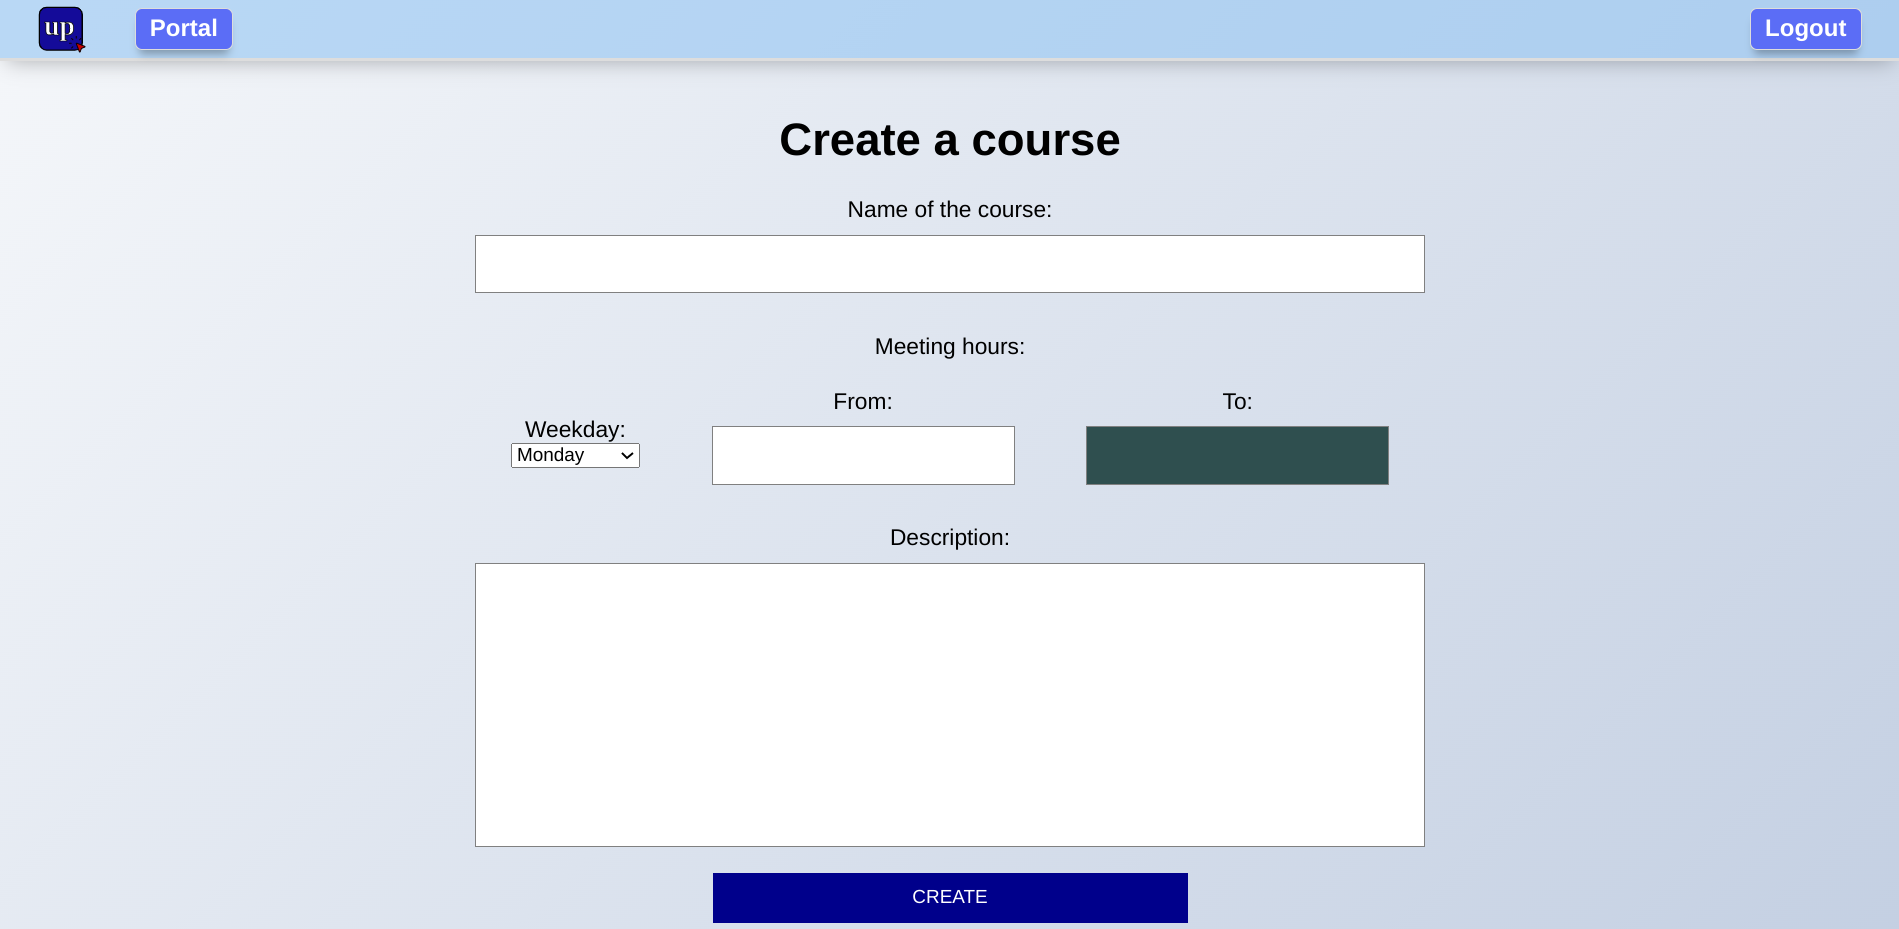
\includegraphics[width=\textwidth]{img/user_manual/professor/create-course-1.png}
    \caption{Screenshot of the course creation page, with an empty form}
\end{figure}

\begin{figure}[H]
    \centering
    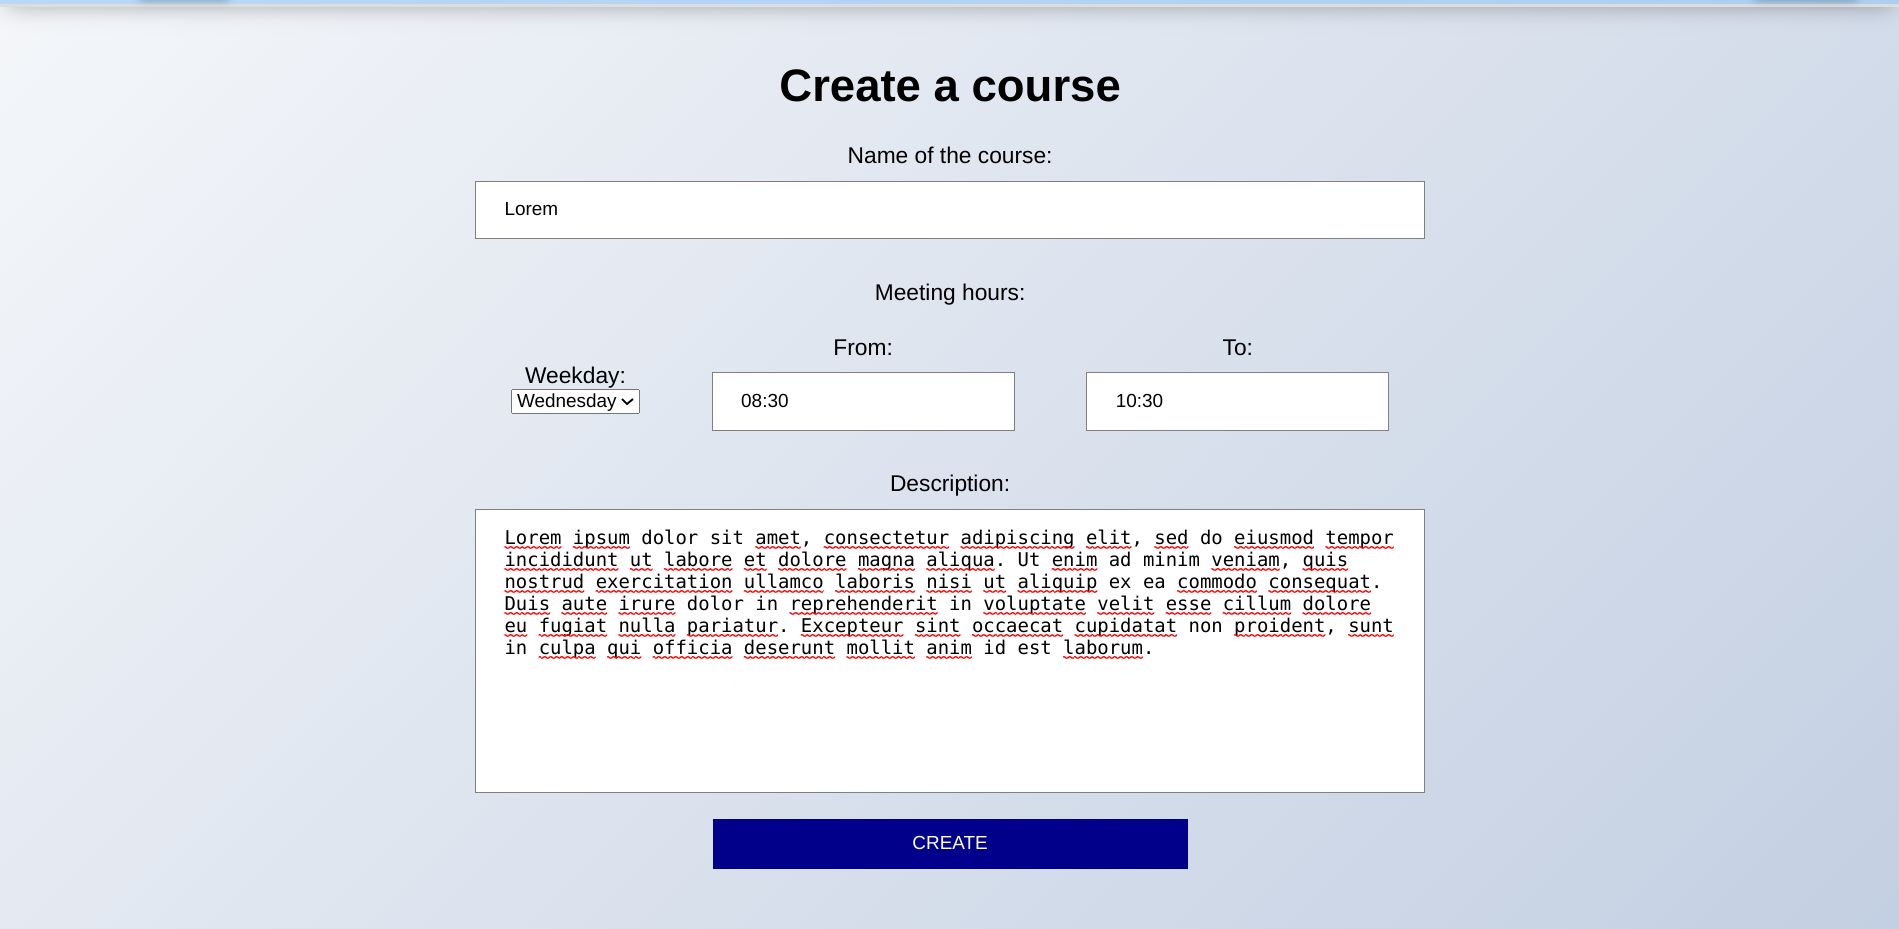
\includegraphics[width=\textwidth]{img/user_manual/professor/create-course-2.png}
    \caption{Screenshot of the course creation page, with a filled form}
\end{figure}

After the professor submits the form, the browser shows an alert pop-up with the result (success/failure) of the course creation.

\begin{figure}[H]
    \centering
    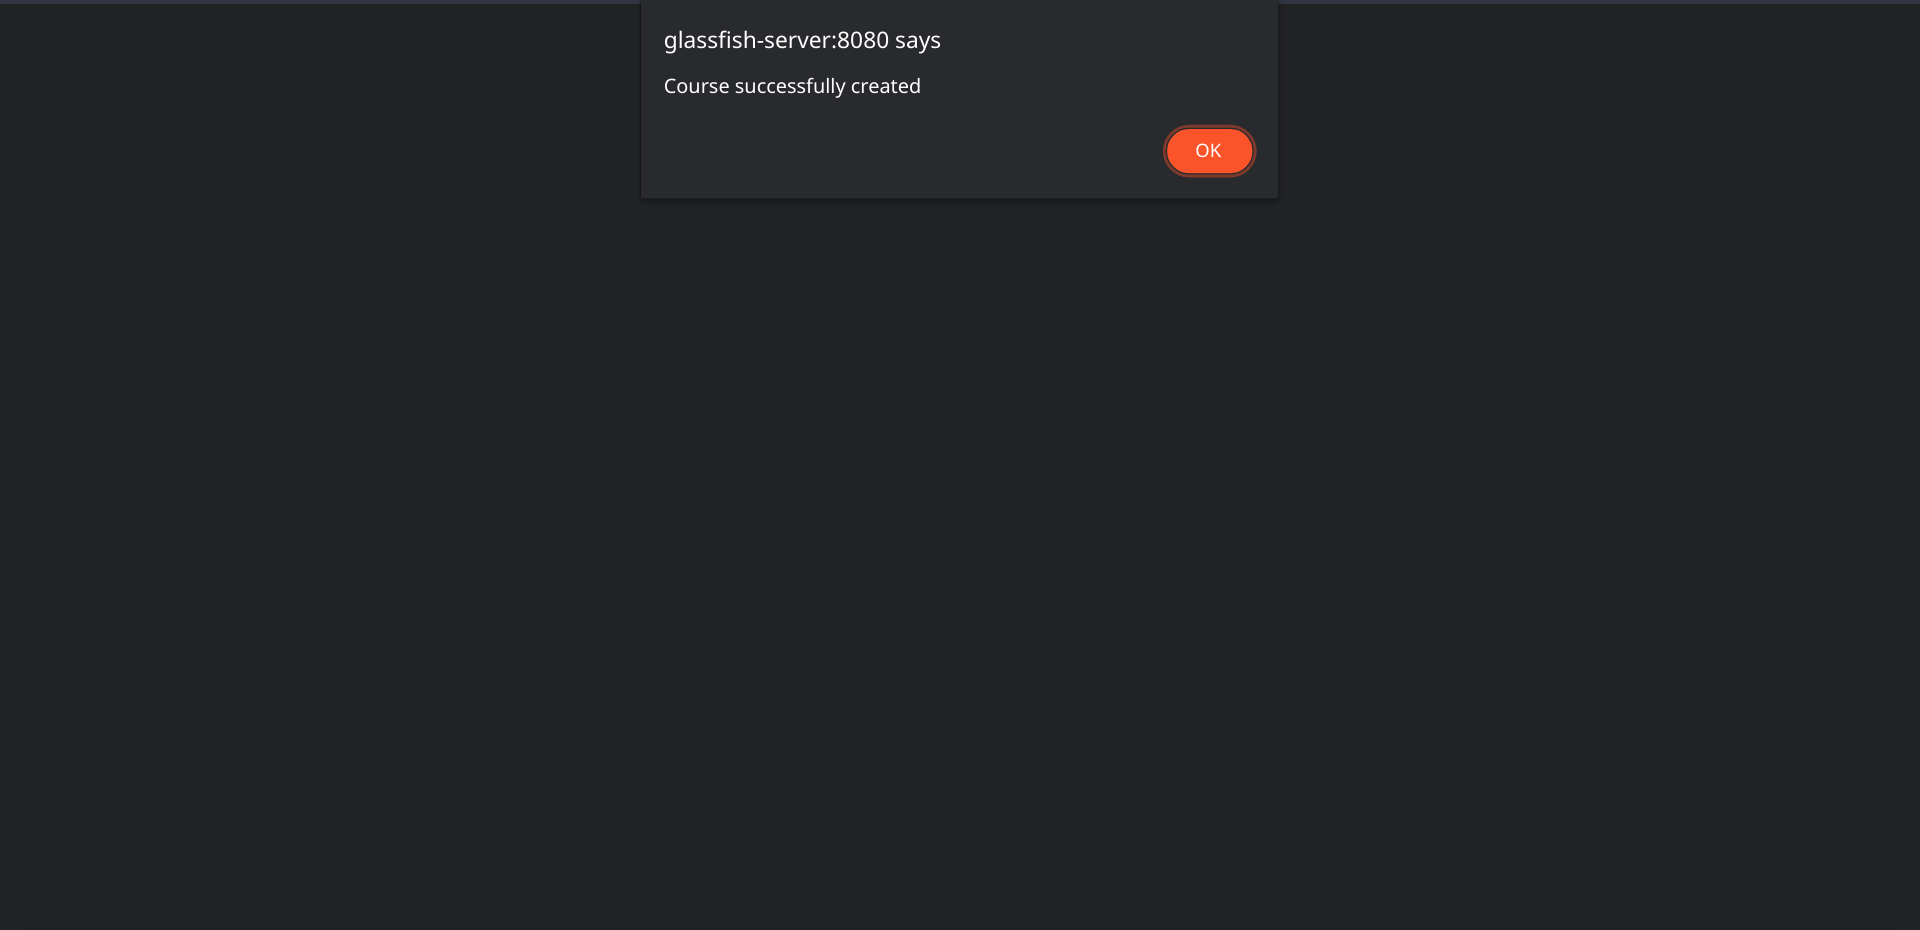
\includegraphics[width=\textwidth]{img/user_manual/professor/create-course-3.png}
    \caption{Screenshot of the course creation page, after the professor submits the form and creation succeeds}
\end{figure}

If the creation succeeds, every student will be able to view the course details page and book a meeting in the available time slots.

\begin{figure}[H]
    \centering
    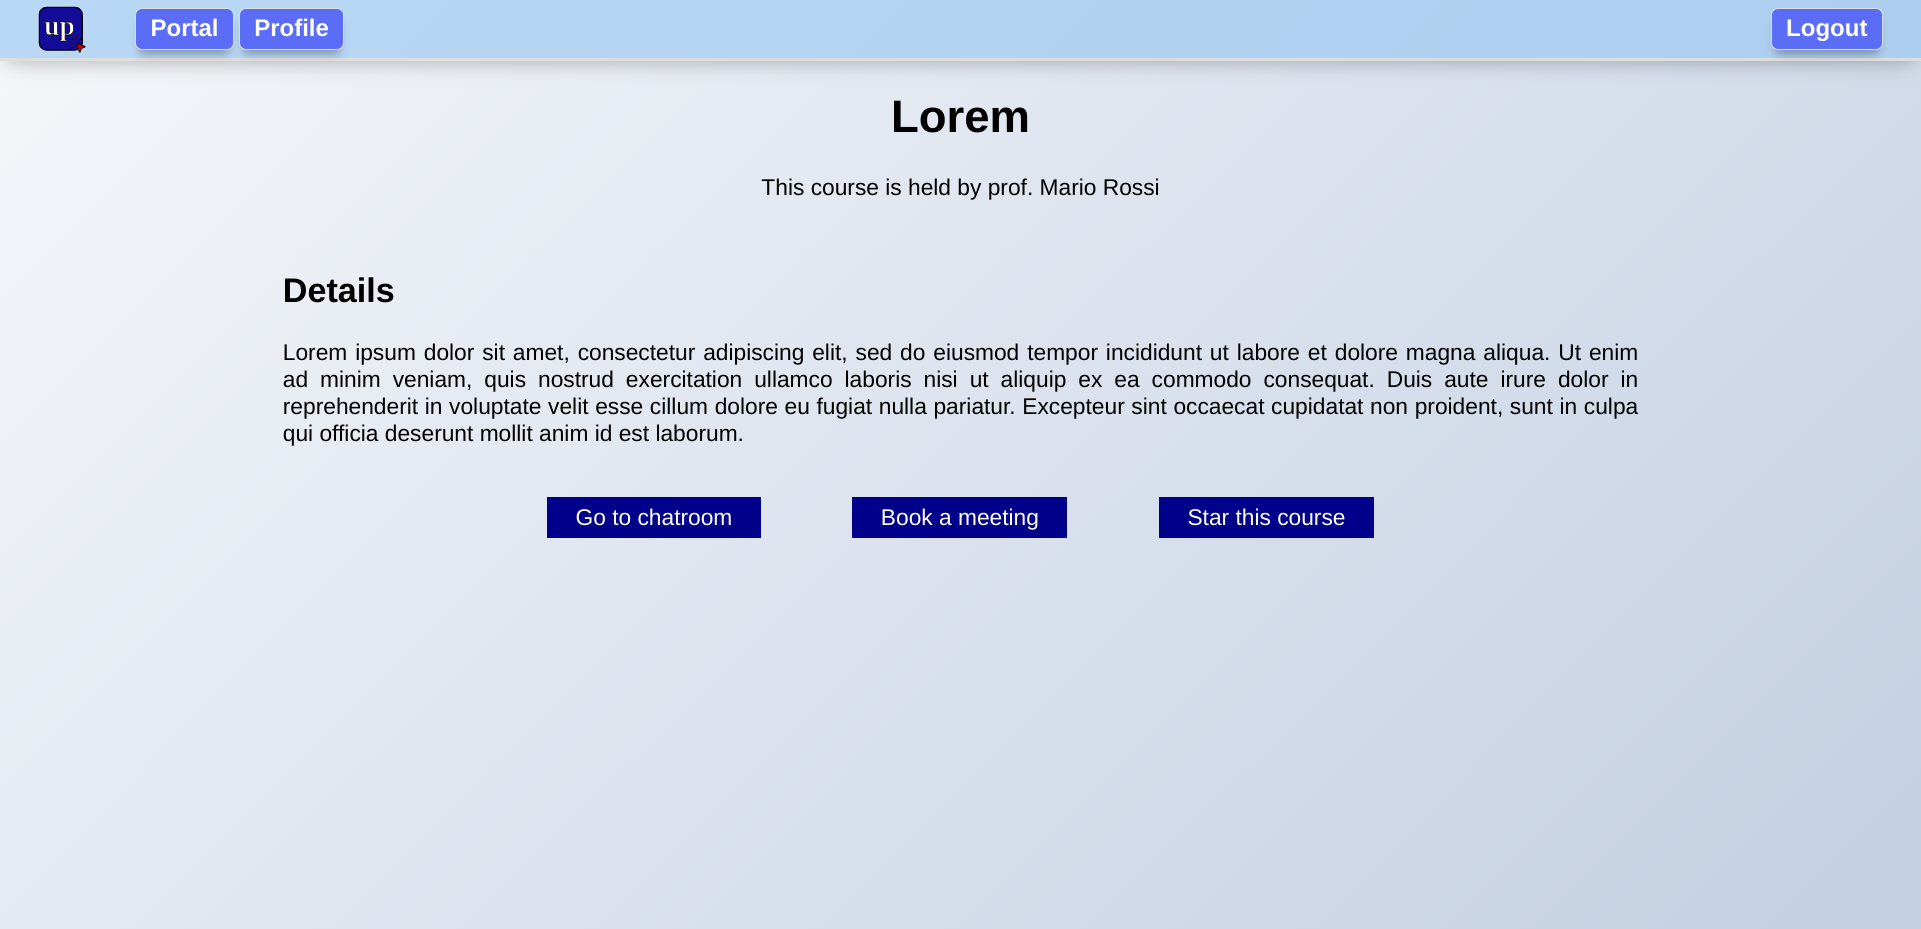
\includegraphics[width=\textwidth]{img/user_manual/professor/create-course-4.png}
    \caption{Screenshot of the course detail page, after the creation of the course}
\end{figure}

\begin{figure}[H]
    \centering
    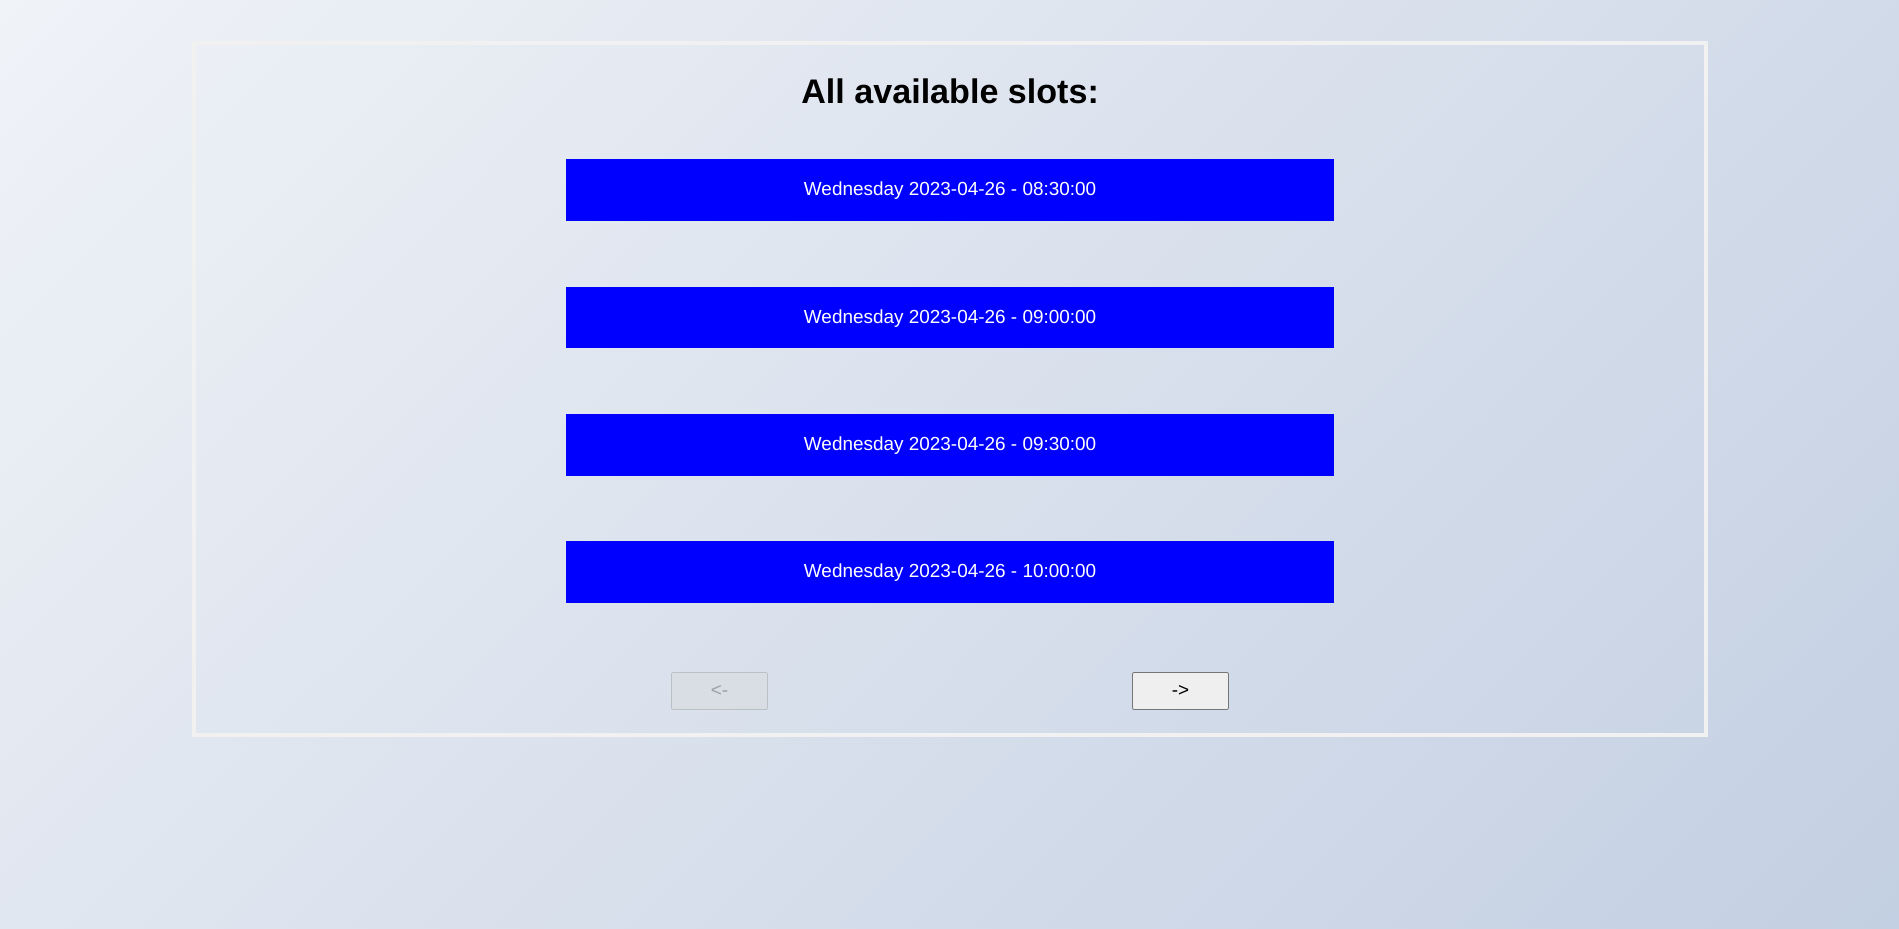
\includegraphics[width=\textwidth]{img/user_manual/professor/create-course-5.png}
    \caption{Screenshot of the page for booking a meeting, after the creation of the course}
\end{figure}


\newpage

\subsection{Show booked meetings}
In this page the professor can see its scheduled meetings and cancel them.\\
The professor can either:
\begin{itemize}
    \item Delete a meeting: by clicking on the corresponding button 
    \item change month of the shown meetings: by clicking on the buttons placed under the meetings list 
\end{itemize}
\begin{figure}[H]
    \centering
    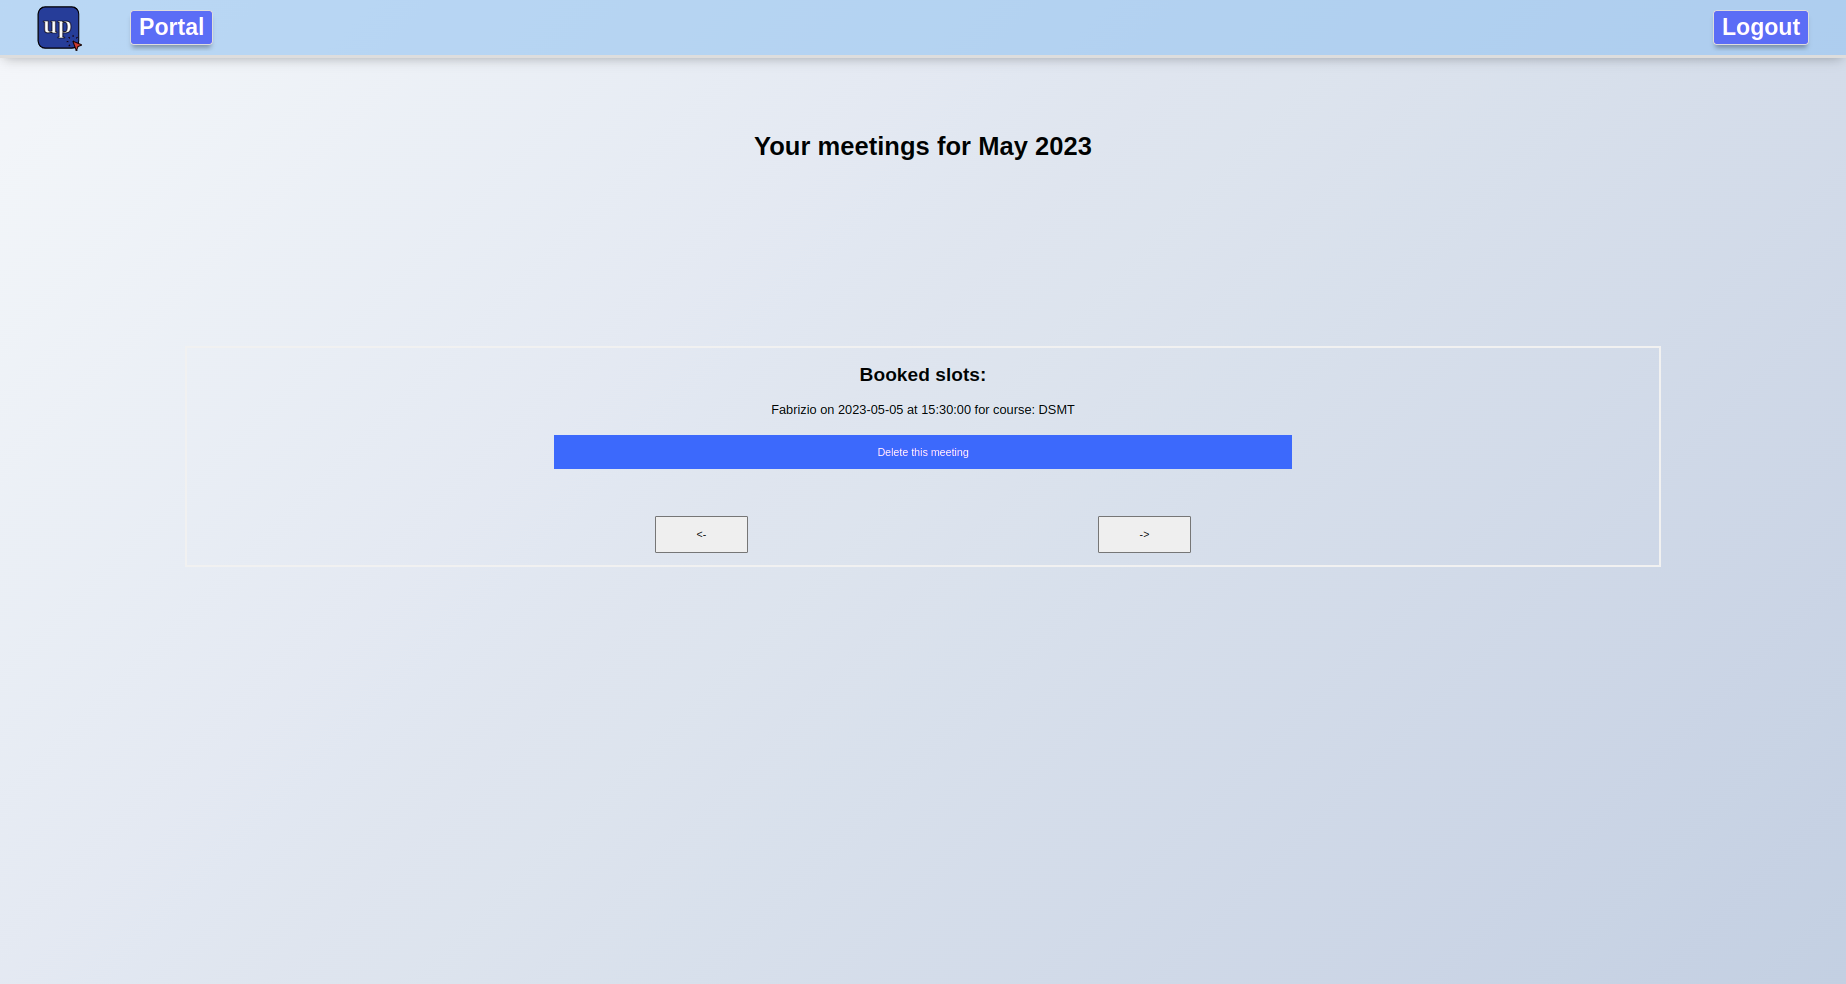
\includegraphics[width=\textwidth]{img/user_manual/professor/Meetings.png}
    \caption{Screenshot of professor/meeting page}
\end{figure}

After the deletion of a meeting the page will show an alert with the operation result.
\begin{figure}[H]
    \centering
    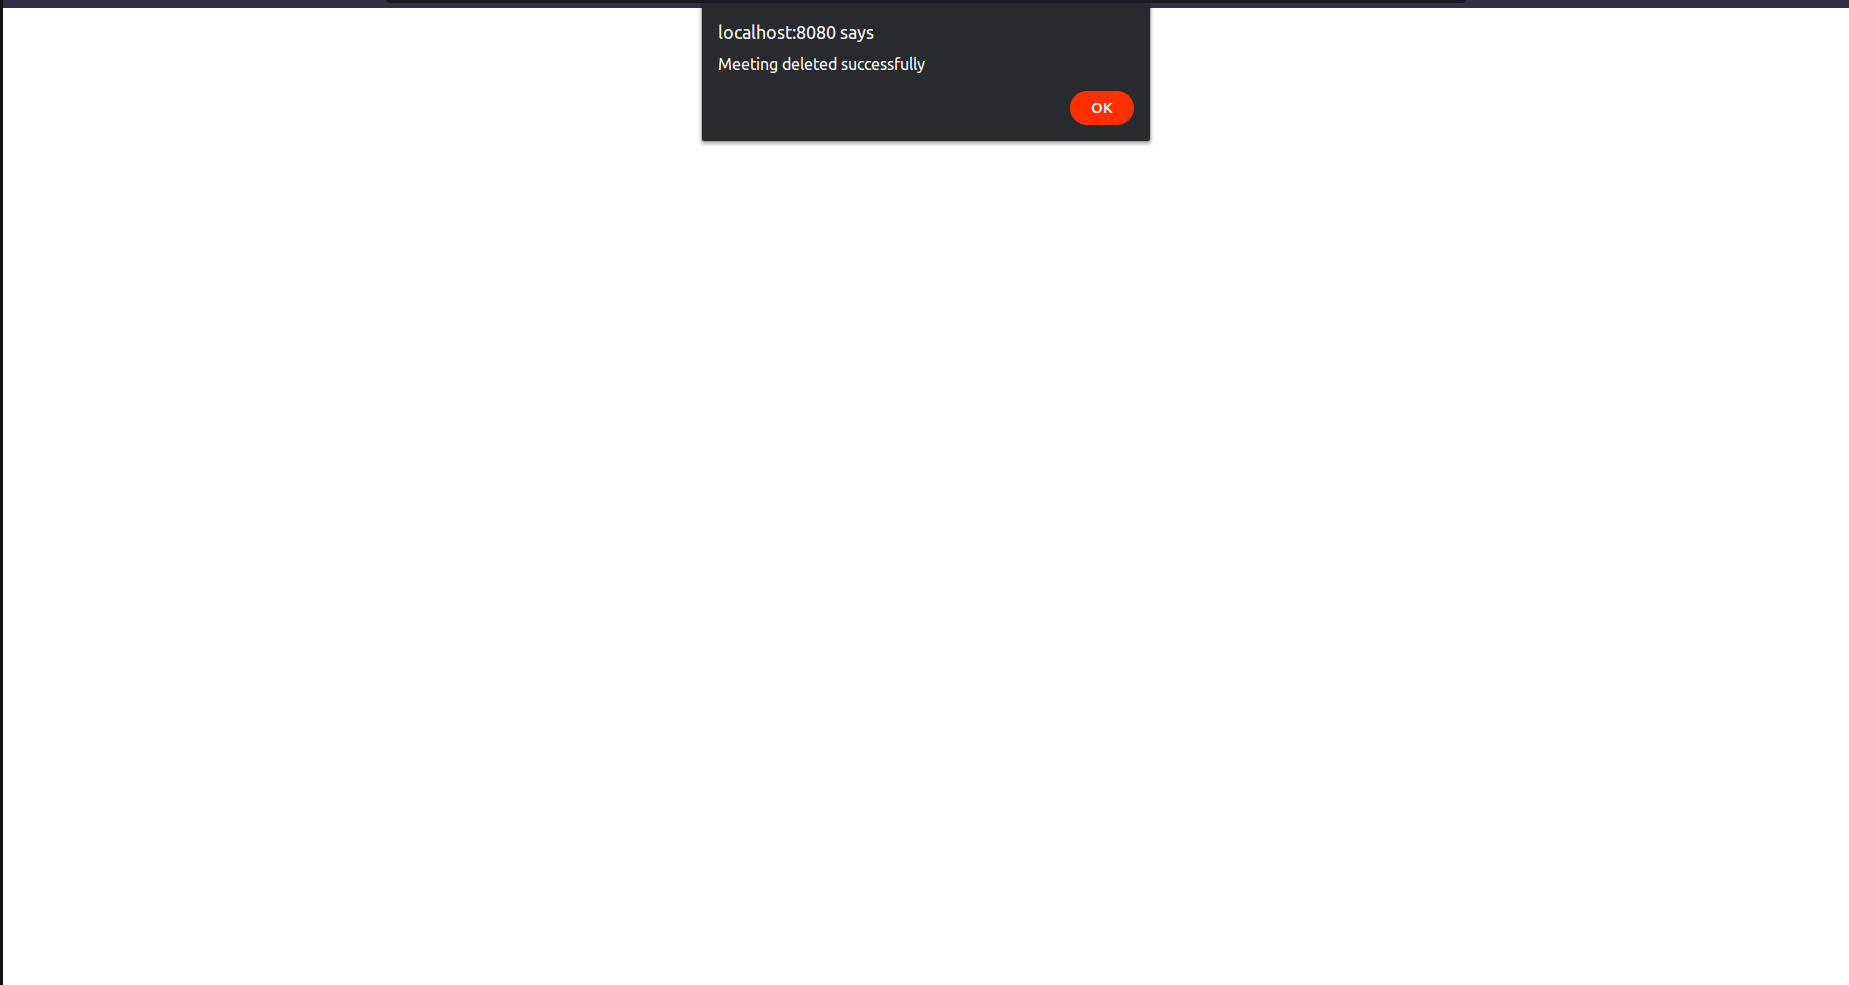
\includegraphics[width=\textwidth]{img/user_manual/professor/meeting-response.png}
    \caption{Screenshot of meeting deletion response}
\end{figure}
\newpage

\subsection{Delete a course} 
This is the delete course page accessible by the professor.\\
The professor can only delete courses that he/she has created.\\
To find the course to delete, he can either search for it through the search bar, or he can browse through all of his courses by hand.\\
Once the course is found, to delete it simply click on the related blue box.\\

\begin{figure}[H]
    \centering
     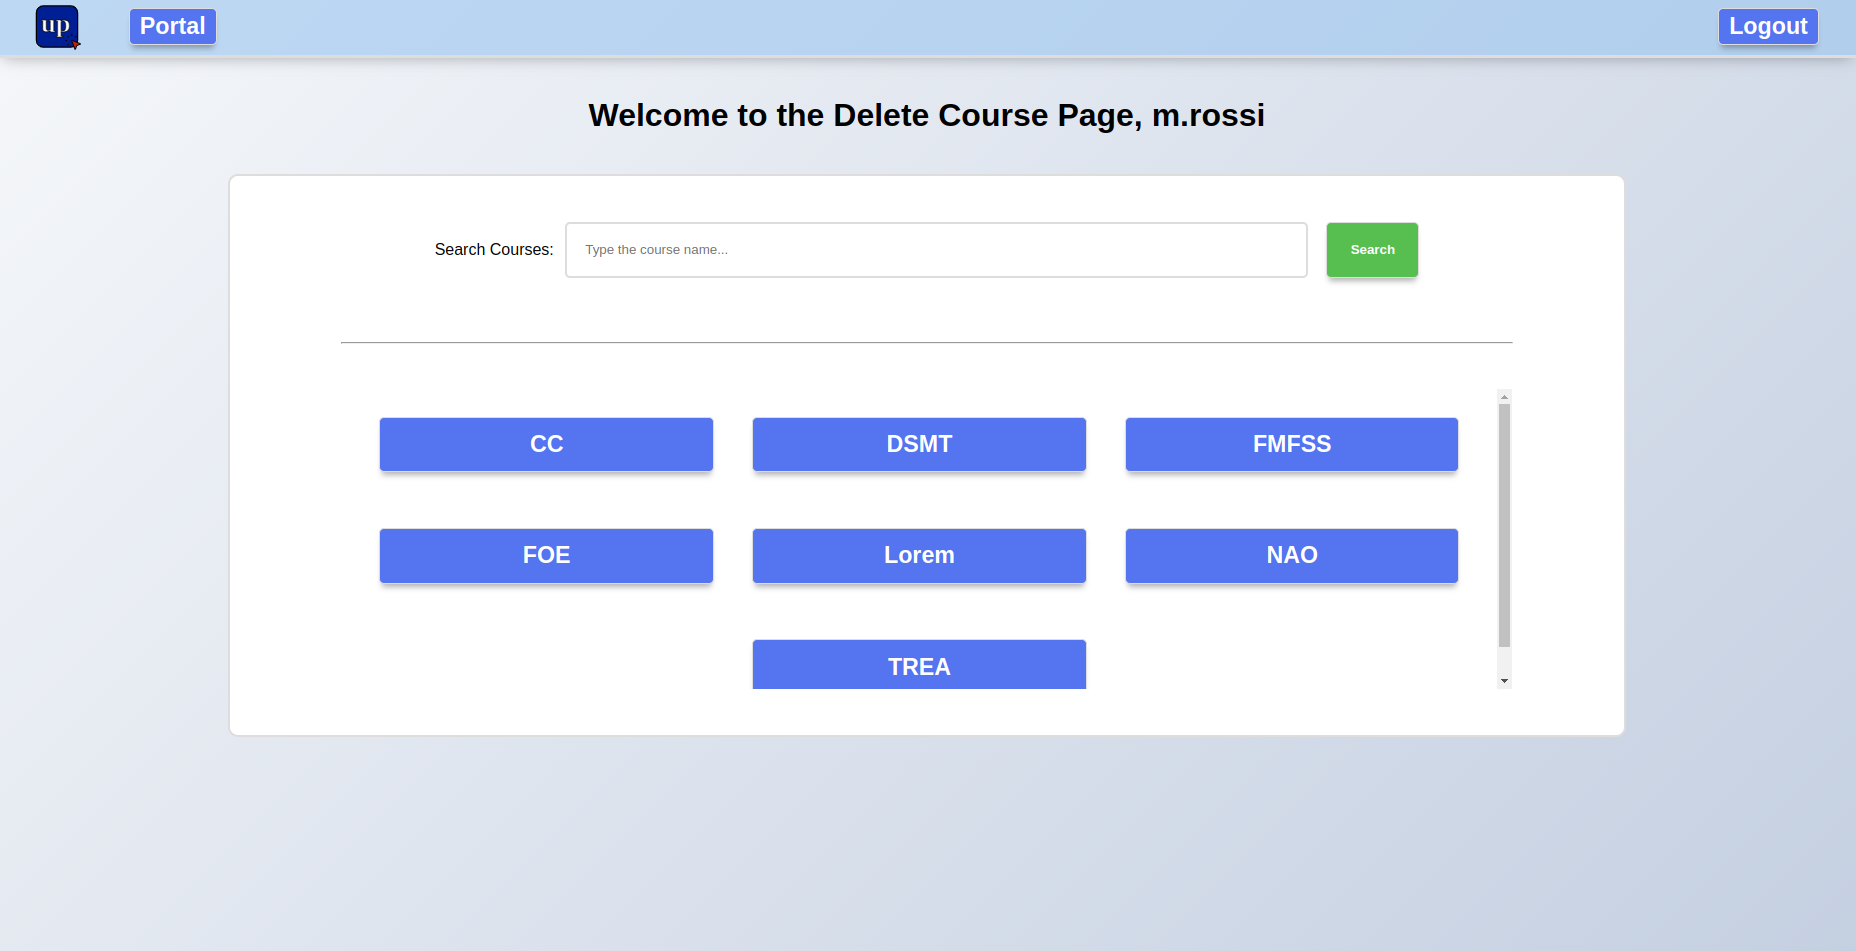
\includegraphics[width=0.95\textwidth]{img/user_manual/professor/delete_course.png}
    \caption{\label{fig:professor-delete-course-1} Screenshot of the delete course page.}
\end{figure}

Immediately after selecting the course to be deleted, an alert pops up and asks for the confirmation for the delete.\\
If the student wants to confirm he/she must click on the delete button otherwise on the x.\\

\begin{figure}[H]
    \centering
     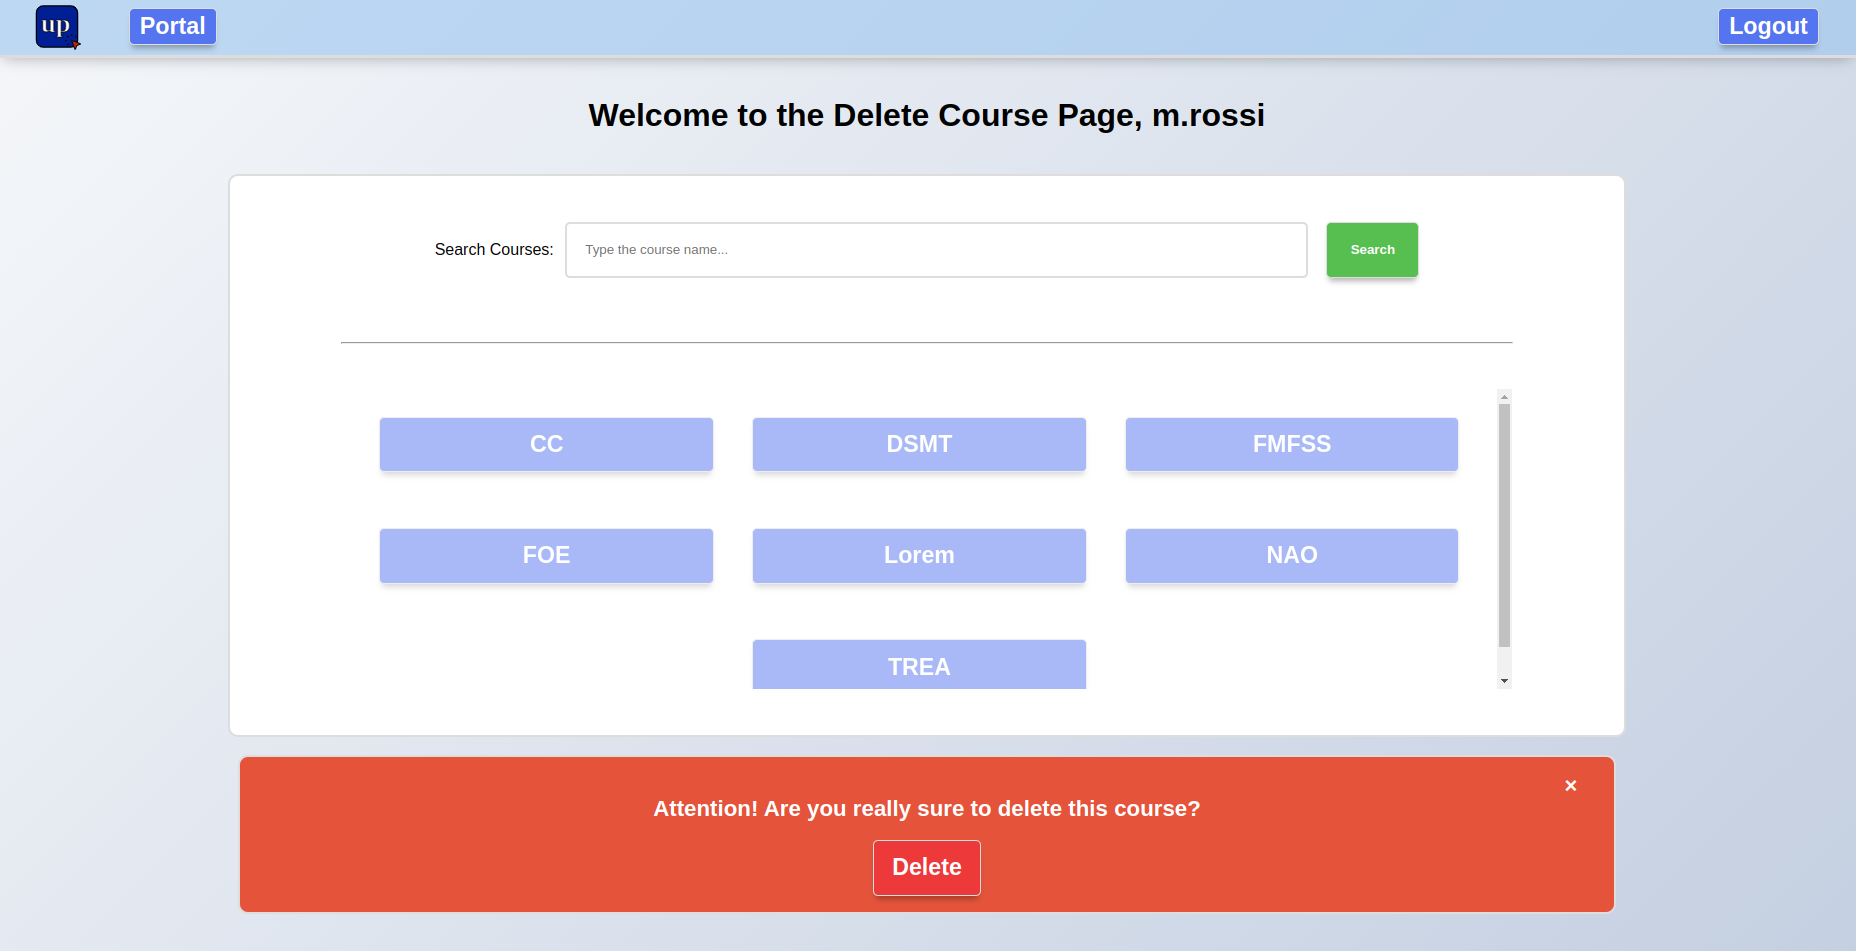
\includegraphics[width=0.95\textwidth]{img/user_manual/professor/delete-course-delete-alert.png}
    \caption{\label{fig:professor-delete-course-2} Screenshot of the delete alert of the delete course page.}
\end{figure}

The page shows a message with the result of the delete operation.

\begin{figure}[H]
    \centering
     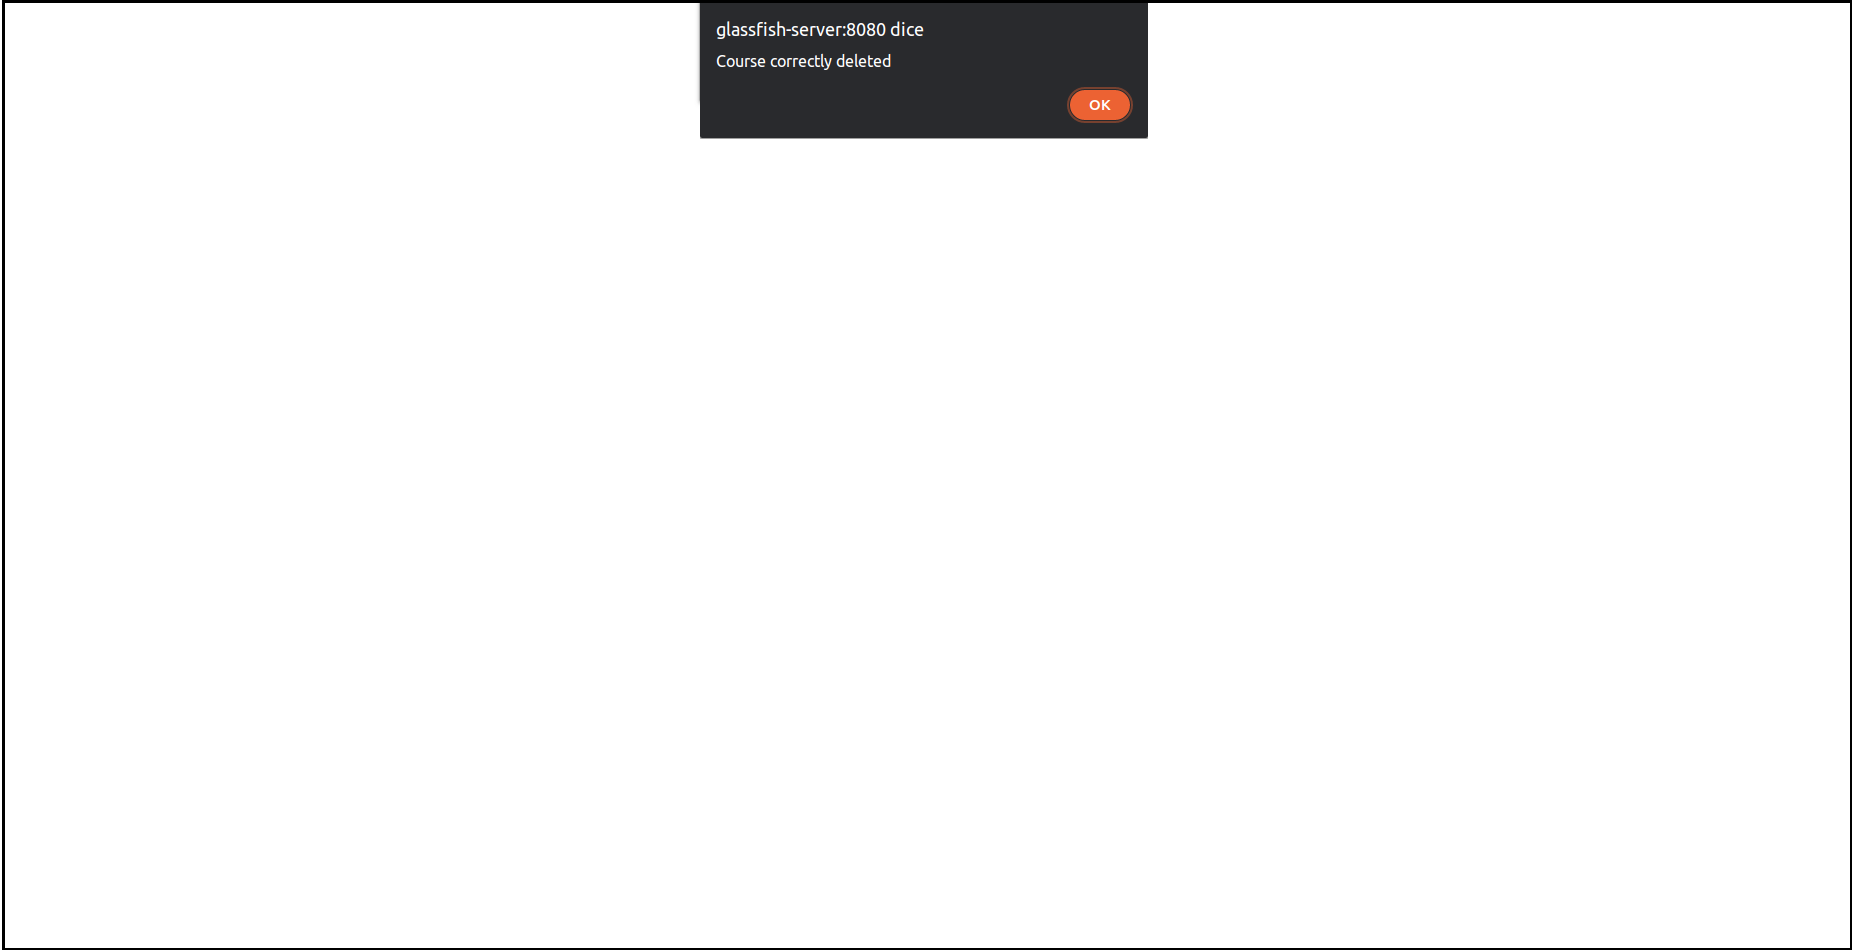
\includegraphics[width=1\textwidth]{img/user_manual/professor/delete-course-alert.png}
    \caption{\label{fig:professor-delete-course-3} Screenshot of the delete course page after the successful delete of the course.}
\end{figure}
\newpage


% ADMIN SECTION
\section{Admin section}

\subsection{Create professor account}
On this page the admin can create a new professor's account.\\
To create this account, simply fill all the fields shown in the figure below and after that, click Create account.\\

\begin{figure}[H]
    \centering
     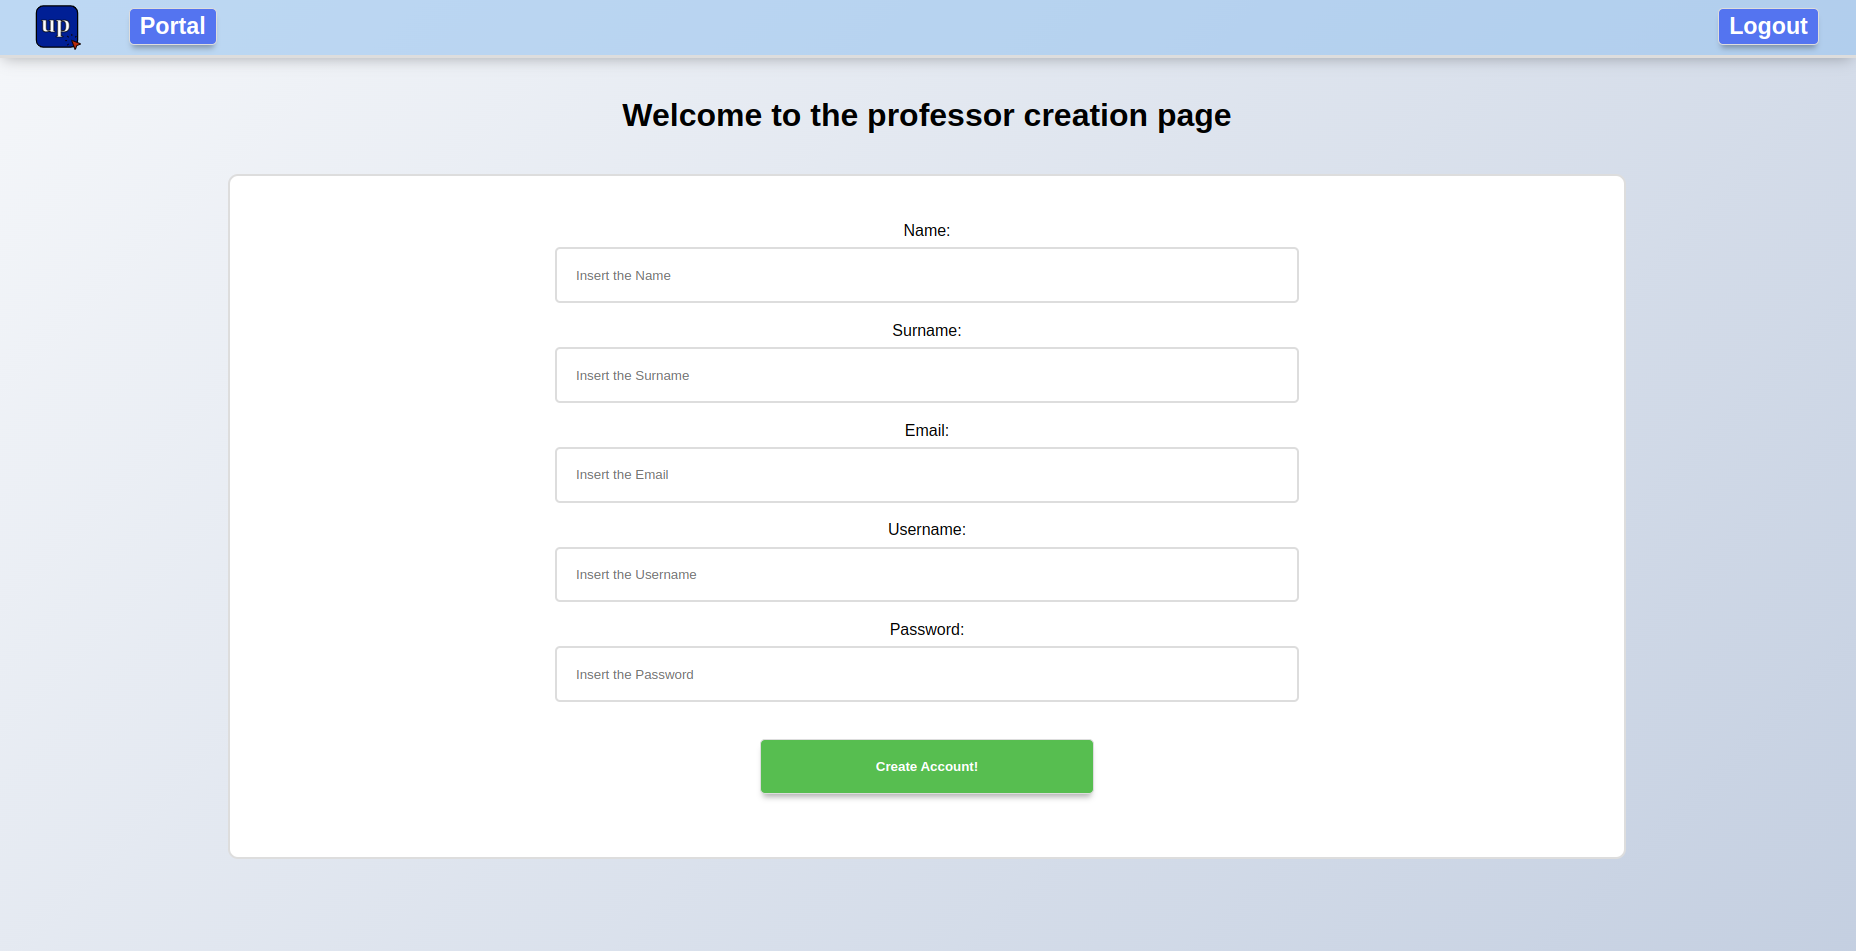
\includegraphics[width=1\textwidth]{img/user_manual/admin/create-professor.png}
    \caption{\label{fig:create-professor} Screenshot of the create professor page.}
\end{figure}

\newpage

\subsection{User browse}
In this page the admin can browse for users and ban them.
The user can either:
\begin{itemize}
    \item Browse users by username: writing in the input field positioned above the user list and by clicking the "Search" button
    \item Switch between the two kind of users: by clicking the button which is either "See professors" or "See students" the admin can switch the user type in which his searches are performed
    \item ban a user: once he found the user that he want, he can ban it clicking on the button with his name
    \item browse the returned list: once he searched for a specific username, he can go through the results clicking on the buttons positioned at the bottom of the page
\end{itemize}
\begin{figure}[H]
    \centering
    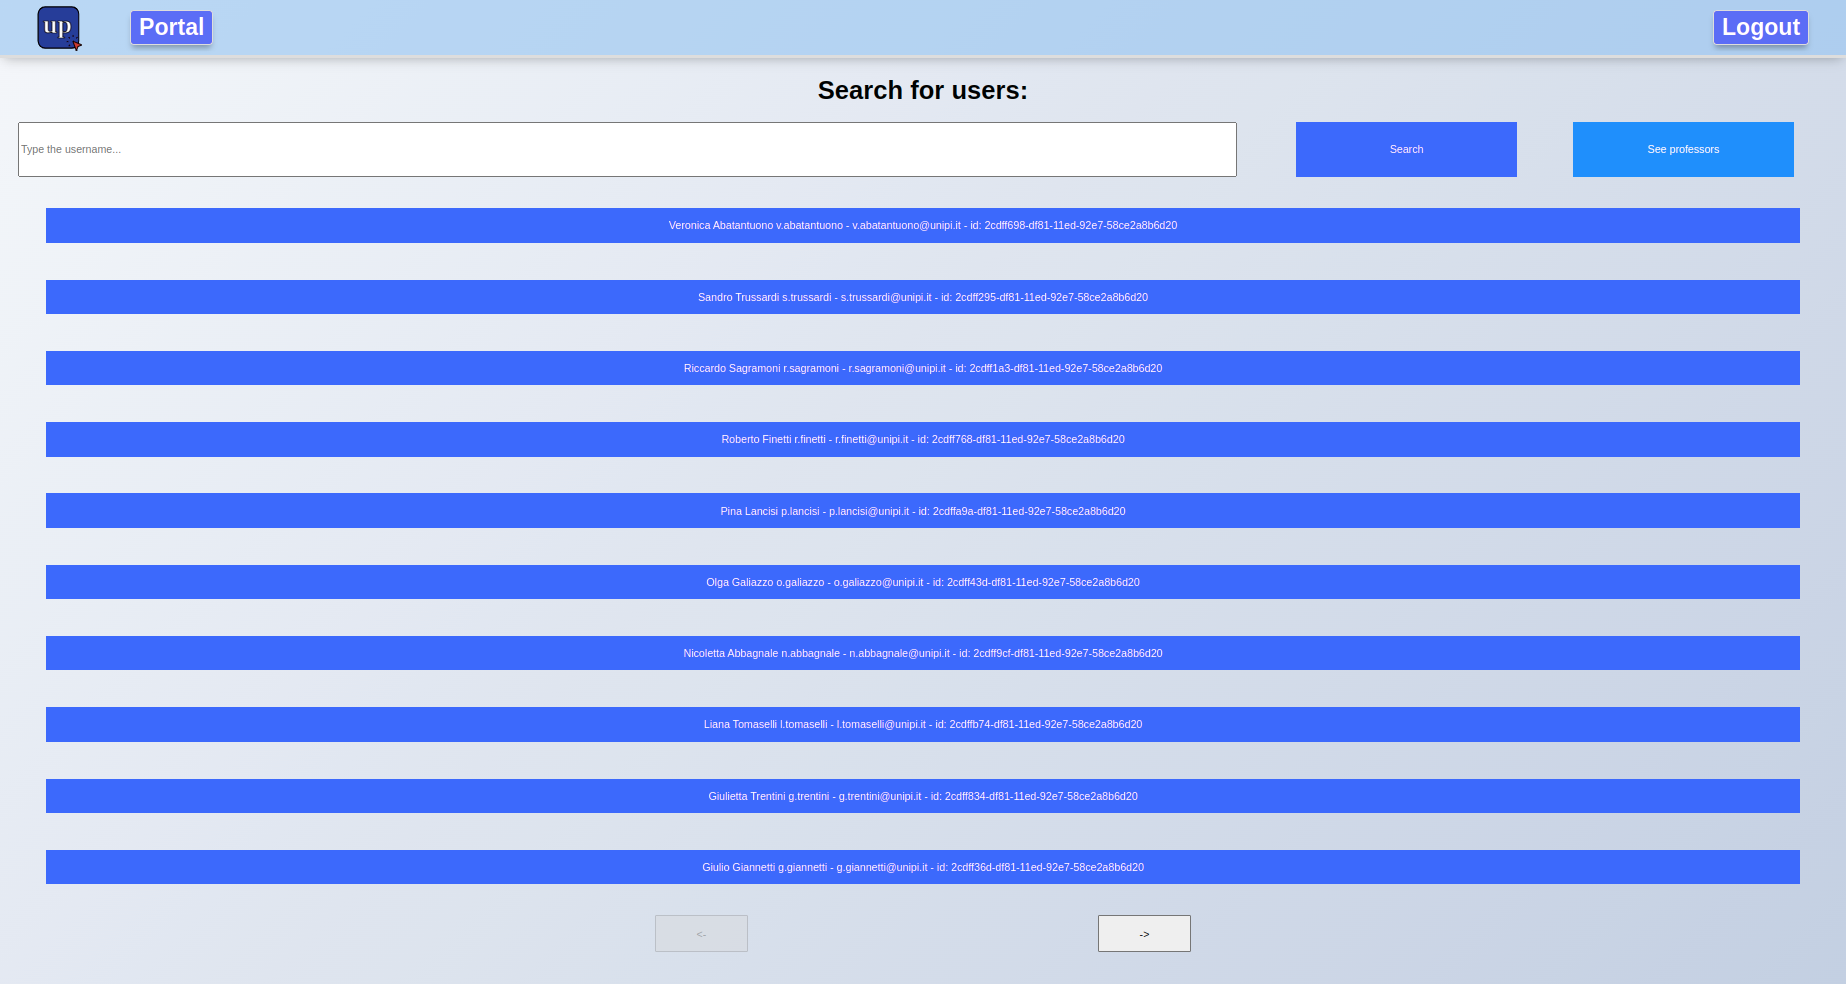
\includegraphics[width=\textwidth]{img/user_manual/admin/admin_search.png}
    \caption{Screenshot of user browsing page}
\end{figure}
After that the admin tried a ban operation an alert will appear to show whether the operation has been successful or not.
\begin{figure}[H]
    \centering
    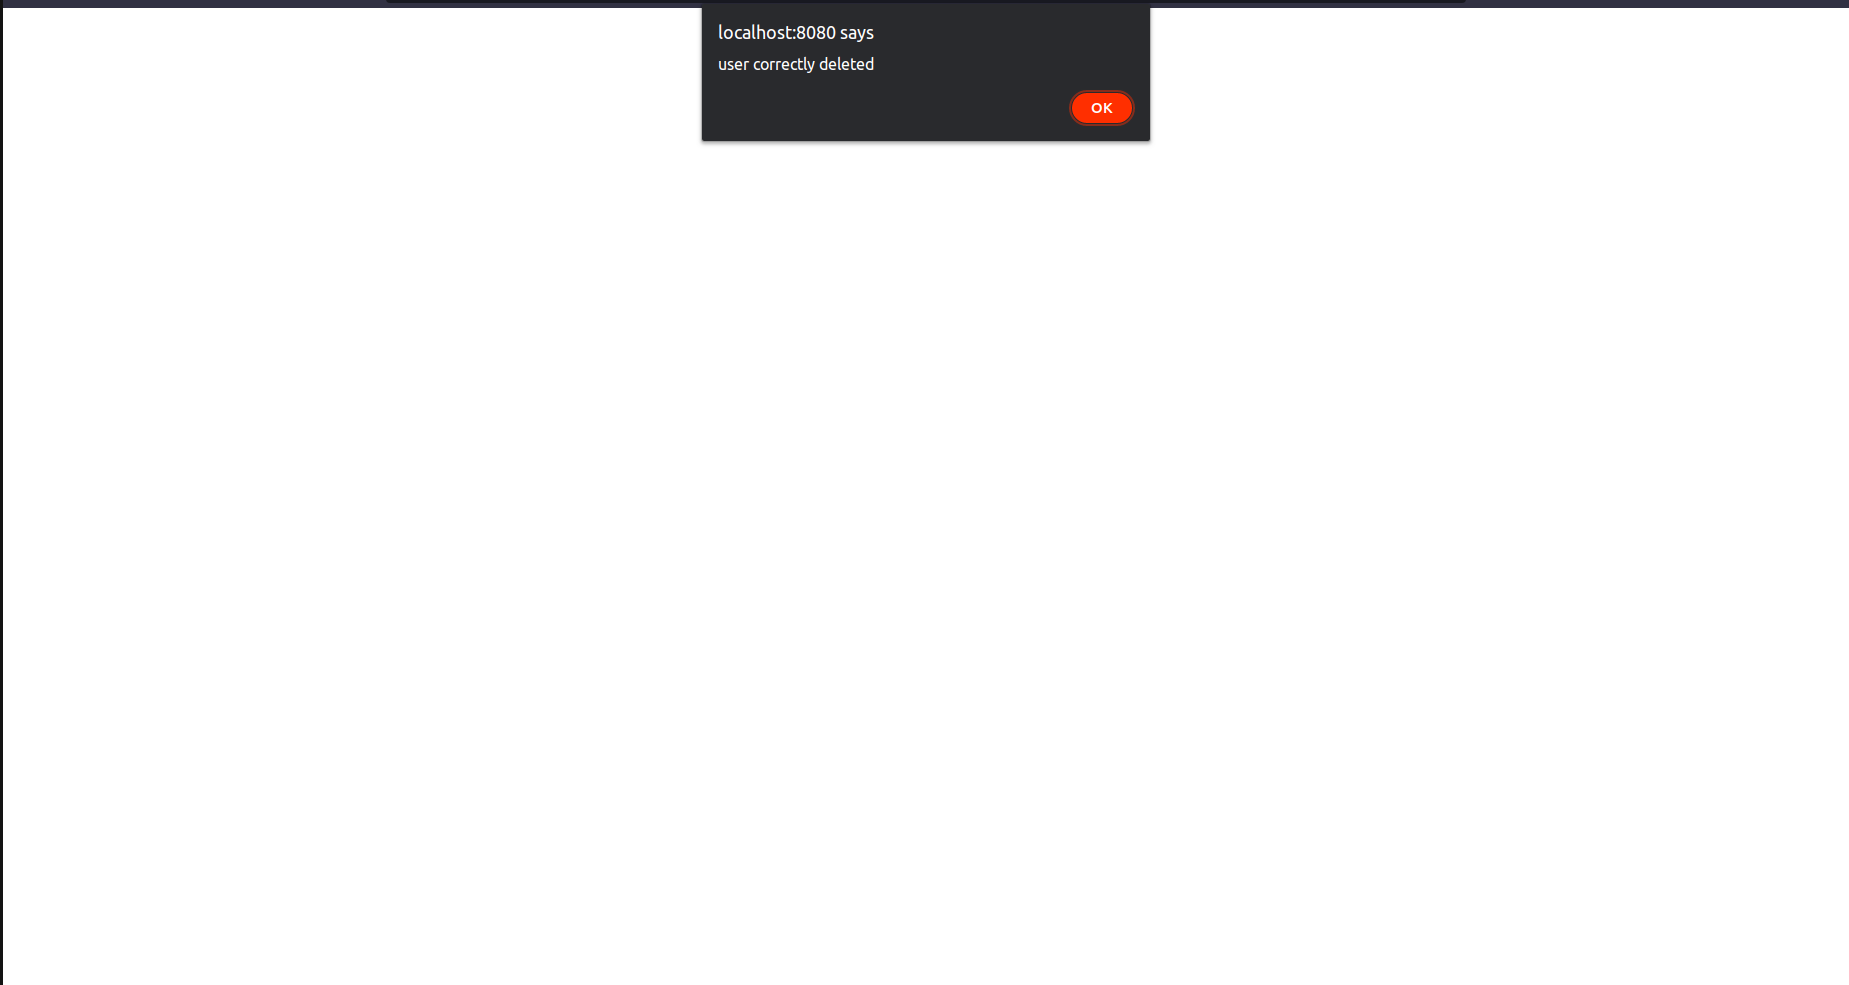
\includegraphics[width=\textwidth]{img/user_manual/admin/ban-response.png}
    \caption{Screenshot of ban response}
\end{figure}

    
\end{document}
